\documentclass{amsart}

\usepackage{amssymb,amsmath,amsthm,amsaddr}
\usepackage{thmtools}
\usepackage{thm-restate}

\usepackage{tikz,pgfplots,pgfplotstable}
\pgfplotsset{compat=1.9} % set to 1.8 to get old behaviour

%% %% % Graphics:
%% \usepackage[final]{graphicx}
\usepackage{graphicx} % use this line instead of the above to suppress graphics in draft copies
\usepackage{wrapfig}
%\usepackage{graphpap} % \defines the \graphpaper command
\usepackage[T1]{fontenc} % Use 8-bit encoding that has 256 glyphs
\usepackage[english]{babel} % English language/hyphenation


\usepackage{cite}
% makes color citations
\usepackage[colorlinks=true,urlcolor=blue,citecolor=red,linkcolor=red,bookmarks=true]{hyperref}
\usepackage{url}
\usepackage{color}
\usepackage{paralist}
%% \usepackage{graphics} %% add this and next lines if pictures should be in esp format
%% \usepackage{epsfig} %For pictures: screened artwork should be set up with an 85 or 100 line screen
\usepackage{epstopdf} 

%% From slides file
\usepackage{booktabs} % Allows the use of \toprule, \midrule and \bottomrule in tables
\usepackage[normalem]{ulem}
\usepackage{xcolor}
%\usepackage{algorithm}
%\usepackage[noend]{algpseudocode}
\usepackage{proof-at-the-end}

% Indent first line of each section:
\usepackage{indentfirst}

%% %% % Fonts and symbols:
\usepackage{amsfonts}


%% % Formatting tools:
%% %\usepackage{relsize} % relative font size selection, provides commands \textsmalle, \textlarger
%% %\usepackage{xspace} % gentle spacing in macros, such as \newcommand{\acims}{\textsc{acim}s\xspace}

%% % Page formatting utility:
%% \usepackage{geometry}
%% %\usepackage[margin=0.1in]{geometry}


%% Place here your \newcommand's and \renewcommand's. Some examples already included.
%\renewcommand{\le}{\leqslant}
%\renewcommand{\ge}{\geqslant}
%\renewcommand{\emptyset}{\ensuremath{\varnothing}}
%\newcommand{\ds}{\displaystyle}
\newcommand{\R}{\ensuremath{\mathbb{R}}}
%\newcommand{\Q}{\ensuremath{\mathbb{Q}}}
%\newcommand{\Z}{\ensuremath{\mathbb{Z}}}
%\newcommand{\N}{\ensuremath{\mathbb{N}}}
%\newcommand{\T}{\ensuremath{\mathbb{T}}}
%\newcommand{\B}{\mathcal{B}}
\newcommand{\eps}{\varepsilon}
%\newcommand{\closure}[1]{\ensuremath{\overline{#1}}}
\newcommand{\M}{\mathcal{M}}

\newcommand{\ep}{\varepsilon}
%\newcommand{\eps}[1]{{#1}_{\varepsilon}}
\newcommand{\bs}{\boldsymbol}
\newcommand{\der}{\text{\textup{d}}}
\newcommand{\coder}[1]{\texttt{#1}}
\newcommand{\inner}[2]{#1 \cdot #2}
\newcommand{\var}{\textup{Var}}
\newcommand{\corr}{\textup{Corr}}
\newcommand{\cov}{\textup{Cov}}
\newcommand{\diag}{\textup{diag}}
%% \newcommand{\dom}{\mathcal{D}om}
%% \newcommand{\note}[1]{{\textcolor{blue}{#1}}}
%% \newcommand{\A}[1]{{\textcolor{cyan}{\noindent Answer: #1}}}
%\newcommand{\reftwo}[1]{{\textcolor{green}{#1}}}
%\newcommand{\refthree}[1]{{\textcolor{red}{#1}}}
%% \newcommand{\refthree}[1]{{\color{red} #1}}
%% \newcommand{\reftwo}[1]{{\color{green} #1}}



%% \newcommand{\precop}{\mathcal{L}}
%% \newcommand{\precmat}{\mathbf{L}}
%% \newcommand{\Op}{\mathcal{A}}
%% \newcommand{\OpDir}{\mathcal{A}_{\textup{Dirichlet}}}
%% \newcommand{\OpNeu}{\mathcal{A}_{\textup{Neumann}}}
%% \newcommand{\covop}{\mathcal{C}}
%% \newcommand{\lag}{\mathcal{L}}
%% \newcommand{\n}{\boldsymbol{n} }
%% \newcommand{\dn}{\partial \n }
\newcommand{\x}{\mathbf{x}}
\newcommand{\y}{\mathbf{y}}
%% \newcommand{\z}{{\boldsymbol{z}}}
%% \newcommand{\kxmy}{ \kappa \| \x - \y \| }
%% \newcommand{\xmy}{ \| \x - \y \| }
%% \newcommand{\proj}{\mathcal{P}}
%% \newcommand{\kr}{\kappa r}
%% \newcommand{\ivar}{\text{IntVar}}

%% \newcommand{\K}{\mathbb{K}}
\newcommand{\hil}{\mathcal{H}}
%% \newcommand{\ban}{\mathcal{B}}
\newcommand{\hilp}{\mathcal{H}_p}
\newcommand{\hilo}{\mathcal{H}_o}
\newcommand{\obs}{\mathcal{O}}
\newcommand{\pobs}{\mathcal{P}}
\newcommand{\fwd}{\mathcal{F}}
%% \newcommand{\tru}{\fwd_{\textup{True}}}
%% \newcommand{\err}{\fwd_{\textup{Error}}}

\newcommand{\obsm}{\widehat{\obs}}
\newcommand{\Sigmam}{\widehat{\Sigma}}
\newcommand{\postcovm}{\widehat{\Gamma_{\textup{post}}}}
\newcommand{\uu}{\mathbf{u}}
\newcommand{\tar}{\Psi}
\DeclareMathOperator*{\argmin}{arg\,min}
\DeclareMathOperator*{\argmax}{arg\,max}

% Definitions for second chapter
\newcommand{\data}{\mathbf{d}}
\newcommand{\param}{\mathbf{m}}
\newcommand{\sspar}{\param_{\textup{SmallScale}}}
\newcommand{\normal}{\mathcal{N}}
\newcommand{\pr}{\mu_{\textup{pr}}} %Prior measure
\newcommand{\post}{\mu_{\textup{post}}^{\data, \obs}} % Posterior measure
\newcommand{\prmean}{\param_{\textup{pr}}} % Prior mean
\newcommand{\postmean}{\param_{\textup{post}}} % Posterior mean
\newcommand{\postcov}{\Gamma_{\textup{post}}} % Posterior covariance
\newcommand{\prcov}{\Gamma_{\textup{pr}}} % Prior covariance
\newcommand{\modcov}{\Gamma_{\textup{model}}} % Model covariance
\newcommand{\tmp}{\mathcal{G}}
\newcommand{\meas}{\mathbf{o}}
\newcommand{\ev}{\mathbf{e}} % eigenvector 
\newcommand{\func}{\mathbf{a}}
\newcommand{\tr}[1]{\textup{tr}\left \{#1 \right \} }
\newcommand{\ttr}[1]{\textup{tr}\ #1}
\newcommand{\rank}{\textup{rank}\ }
\newcommand{\des}{\eta} % vector of design parameters
\newcommand{\sigsqr}{\sigma^2}
%\newcommand{\acim}{\textsc{acim}\xspace}
%\newcommand{\acims}{\textsc{acim}s\xspace}


%% %% \newcommand\numberthis{\addtocounter{equation}{1}\tag{\theequation}}
%% %% %%
%% %% %% Place here your \newtheorem's:
%% %% %%
\newtheorem{theorem}{Theorem}
\newtheorem{definition}{Definition}

%% %% %% Some examples commented out below. Create your own or use these...
%% %% %%%%%%%%%\swapnumbers % this makes the numbers appear before the statement name.
%% %% %\theoremstyle{plain}
%% %% %\newtheorem{thm}{Theorem}[chapter]
\newtheorem{proposition}{Proposition}
\newtheorem{lemma}{Lemma}
\newtheorem{corollary}{Corollary}
%% %% % \newtheorem{observation}[theorem]{Observation}

%% %% %\theoremstyle{definition}
%% %% %\newtheorem{define}{Definition}[chapter]

%% %% %\theoremstyle{remark}
%% %% %\newtheorem*{rmk*}{Remark}
%% %% %\newtheorem*{rmks*}{Remarks}

%% %% %% Hack
%% %% \newcommand{\stkout}[1]{\ifmmode\text{\sout{\ensuremath{#1}}}\else\sout{#1}\fi}
%% %% \usepackage{cancel}

\usepackage{comment}% http://ctan.org/pkg/comment
%% %% %\excludecomment{proof}
%% \excludecomment{figure}
%% \let\endfigure\relax


\overfullrule=0pt


\numberwithin{equation}{section}

\begin{document}

\title[Sensor Clusterization in D-optimal design in infinite
  dimensions]{Sensor Clusterization in D-optimal Design in Infinite
  Dimensional Bayesian Linear Inverse Problems}

\author{Yair Daon}
\address{Porter School of the Environment and Earth
  Sciences, Tel Aviv University\\ Tel Aviv, Israel}
%% \curraddr{Porter School of Environment Studies, Tel Aviv University\\ Tel Aviv, Israel}
%% \curraddr{}
\email{yair.daon@gmail.com}
%% \thanks{}

%    The 2010 edition of the Mathematics Subject Classification is
%    the current definitive version.
\subjclass{Primary: 
  62F15, % Statistics - bayesian inference
  35R30, % PDE - Inverse problems
  Secondary:
  28C20, % Measure and integration - set functions and measures and integrals in
  %infinite-dimensional spaces (Wiener measure, Gaussian measure, etc.
}
%% Primary: 62F15, 35R30; Secondary: 28C20
\date{\today}

\begin{abstract}
  We investigate the problem of sensor clusterization in D-optimal
  experimental design for infinite-dimensional Bayesian linear inverse
  problems. We suggest an analytically tractable model for such
  designs and reason how it may lead to sensor clusterization in the
  case of iid measurement noise. We also show that in the case of
  spatially correlated measurement error clusterization does not
  occur. As a part of the analysis we prove a Matrix Determinant Lemma
  in Hilbert spaces and a lemma for calculating $\frac{\der}{\der t}
  \log \det (I + X(t))$ for certain operator-valued functions. We also
  show how to decompose $M = AA^t$ with $A$ constrained to have unit
  norm columns.
\end{abstract}

\maketitle

\section{Introduction}\label{section:OED intro}
Experimental design is an important part of many scientific
investigations. When considering an inverse problem, one can often
specify sensor locations (e.g.\ in geophysics and oceanography
applications), certain wavelengths (e.g.\ in MRI) or wave reflections
from the ground (e.g.\ searching for oil or using a radar). Whatever
the allowed set of measurements is, one should select the optimal
measurements to take, in order to increase accuracy, reduce costs, or
both.

Designing experiments is usually done by optimizing some \emph{design
  criterion}. This is true both for frequentists
\cite{Silvey13,Ucinski05} as well as for Bayesians
\cite{ChalonerVerdinelli95}. See \cite{ChalonerVerdinelli95} for an
investigation of the analogy between the two approaches. Although
there is a plethora of design criteria, we focus on just one of these,
commonly referred to as \emph{D-optimal design}. It has a simple and
appealing motivation in the Bayesian context as explained in
\cite{ChalonerVerdinelli95}: A D-optimal design seeks to maximize the
expected information gain (KL divergence
\cite{KullbackLeibler51,CoverThomas12}) between posterior and
prior. For example, consider a linear model in finite dimensions, with
Gaussian prior and noise. In this model, maximizing the expected
information gain amounts to minimizing the determinant of the
posterior covariance matrix. In a frequentist setting, a D-optimal
design minimizes the volume of the uncertainty ellipsoid \cite[page
  16]{Ucinski05}, but this is done for the Fisher information matrix
and not the posterior covariance. However, \cite{ChalonerVerdinelli95}
show that the latter is just a regularized version of the former.

The previous discussion is classical for experimental design when
inference is to take place over a finite (not too large) number of
parameters. The subject of optimal experimental design for function
inference in a Bayesian context was pioneered by
\cite{AlexanderianGloorGhattas14, AlexanderianPetraStadlerEtAl16,
  AlexanderianPetraStadlerEtAl14}. Similarly to the finite dimensional
case, it can be shown that a D-optimal design arises naturally for
linear models when one wishes to maximize the KL divergence between
posterior and prior. This amounts to minimizing the determinant of the
posterior covariance operator (understood as a product of its
eigenvalues). Some difficulties arise in the process, but remedies can
be found as shown in \cite{AlexanderianGloorGhattas14}.

It seems counter intuitive that when one computes an optimal design
using the D criterion, the optimization process results in
measurements that are very similar. For example, if a measurement is
thought of as measuring some function value at $\x \in \Omega
\subseteq \R^d, d=1,2,3$ (with added error) then the optimization
procedure sometimes places sensors in very close proximity to each
other (as can be seen in figure \ref{fig:clusterization
  illustration}). Following \cite{Ucinski05}, we refer to this
phenomenon as \emph{sensor clusterization}.

\subsection{Related Work}
The phenomenon of sensor clusterization seems to be known in several
different contexts. In a frequentist and finite-dimensional context,
\cite{Fedorov96} and \cite[chapter 2.4.3]{Ucinski05} discuss this
phenomenon and suggest an approach called clusterization-free design.
In such designs, the user enforces measurement locations to be far
from each other. One way to do this is by introducing correlated
errors which, philosophically, accounts for both measurement error and
model error. Another method considered is imposing distance
constraints between measurements. A somewhat different approach is
suggested in \cite[page 49]{Fedorov12}, where close by design
measurements are merged --- a procedure which obviously does not avoid
clusterization. The same problem arises in time-series analysis for
pharmacokinetic experiments. The authors of \cite{Hooker09} suggest
modeling auto-correlation time in the noise model, which is equivalent
to the correlated errors mentioned above.

Any of the above mentioned approaches might serve as a remedy and push
sensors away from each other. Yet, none offers any insight as to why
clusterization occurs. Also, as better models are employed, model
error is decreased and the clusterization phenomenon will eventually
reappear. While these approaches are practical and help us avoid the
problem, they do not provide insight as to why sensors are clustering.

In the inverse problems community, work is mostly computational and
less theoretic. Model errors were considered in \cite{Attia20,
  Koval20}. The former study is focused on inferring of a Quantity of
Interest (QoI). The focus of the latter is reducing forward solves,
using randomized linear algebra. Both studies present numerical
techniques for finding optimal designs when model error is
present. Both are restricted to linear inverse problems (although in
the latter the authors use their method on a nonlinear problem by
taking a Laplace approximation for the posterior). Both find an
optimal design by first solving a continuous problem for sensor
weights. Said solution is then sparsified to give a binary
design. Both studies are successful in the task of Bayesian
inversion. However, neither of these studies mentions any effect model
errors can have on sensor clusterization. The current study is mostly
theoretical and aims to fill the theoretical gap of understanding
sensor clusterization.


\subsection{Contribution}
We propose and thoroughly study a relaxed and analytically tractable
model for understanding D-optimal designs. In this model, D-optimal
design are solutions of a constrained optimization problem, formulated
using Lagrange multipliers (section \ref{section:D and grad}). Using
this model we rigorously show how model error mitigates clusterization
(section \ref{section:non vanishing}). We show how clusterization
occurs in a sequential design scenario (section
\ref{subsec:clusterization sequential}). Then, we consider a
simultaneous D-optimal design scenario (section
\ref{subsec:clusterization simultaneous}). We show that designs that
exhibit clusterization are just as optimal as clusterization free
designs.

A beautiful mathematical structure arises in D-optimal designs when no
model error is present. The Lagrange multipliers problems is in fact a
nonlinear eigenvalue problem for the observations and prior
covariance. The operator for which eigenvectors and eigenvalues are
sought is a sum of two operators. The first is the prior
covariance. The second is an outer product of the observations (see
\eqref{eq:eigenproblem} for details and exact statement). This
structure helps us shed light into D-optimal designs. We characterize
these designs using Theorem \ref{thm:char}. One insight we prove in
said theorem, is that a D-optimal design reduces uncertainties where
they are highest first. Other interestig phenomena arise, but they
require setting notation, and are discussed later.

In the process we generalize several lemmas from linear algebra to
infinite-dimensional settings. We prove a Matrix Determinant Lemma in
\ref{lemma:MDL}. We generalize a lemma due to Lax \cite{lax97} for
calculating $\frac{\der}{\der t} \log \det (I + X(t))$, for an
operator valued function $X(t)$ in \ref{lemma:lax}. We also prove
lemmas in linear algebra. One gives a decomposition $M = AA^t$ where
$A$ has unit norm columns \ref{lemma:free}. Another shows simultaneous
diagonizability of the prior and outer product in the nonlinear
eigenvalue problem referenced above \ref{lemma:sim diag}. We also
provide other tools for understanding D-optimal designs in
infinite-dimensional Bayesian inverse problems, including lemmas for
calculating the increase in the design criterion per observation ---
Lemma \ref{lemma:design increase} and Corollary \ref{cor:zero mod
  err}.


\subsection{Limitations}\label{subsec:limitations}
There are two main drawbacks of the study presented here. Our relaxed
model does not consider any specific set of allowed
measurements. Rather, we take measurements in the unit ball in some
Hilbert space. This allows considerably less restrictive observations
than any real-life problem does. The second drawback is that we do not
show rigorously that clusterization necessarily occurs in a
simultaneous design. We only show that it is as reasonable as no
clusterization.


\subsection{An Example of Clusterization}\label{subsec:example}
\begin{figure}
  \begin{tikzpicture}[thick, scale=1.3, every node/.style={scale=0.99}]
    \begin{axis}
      [
      title={Posterior Pointwise Standard Deviations and D-Optimal Sensor Locations},  
      xmin = 0,
      xmax = 3.14,
      xlabel = {$x$},
      ylabel = posterior std,
      ymin   = 0,
      %compat = 1.3,
      % ymax   = 130,
      % ytick = \empty,
      legend cell align=left,
      % legend style={at={(0.45,0.2)}}
      legend pos= outer north east 
      ]
      % \draw[black!30!white, thin] (50,0) -- (50,130);
      % 
      %% \addplot [thin, black, mark=none] table{stdv-heat-sens1-var1.txt};
      %% \addlegendentry{1 sensors};
      
      %% \addplot [thin, blue, mark=none] table{stdv-heat-sens2-var1.txt};
      %% \addlegendentry{2 sensors};
      
      %% \addplot [thin, red, mark=none] table{stdv-heat-sens3-var1.txt};
      %% \addlegendentry{3 sensors};
      
      \addplot [thin, green, mark=none] table{stdv-heat-sens4-var1.txt};
      \addlegendentry{4 sensors};
      
      \addplot [thin, purple, mark=none] table{stdv-heat-sens5-var1.txt};
      \addlegendentry{5 sensors};
      
      \addplot [thin, cyan, mark=none] table{stdv-heat-sens6-var1.txt};
      \addlegendentry{6 sensors};

  
      %% \addplot [black,  only marks, mark=x, mark size=1.5] 
      %% table{locs-heat-sens1-var1.txt}; 
      %% \addplot [blue,   only marks, mark=x, mark size=1.5]
      %% table{locs-heat-sens2-var1.txt}; 
      %% \addplot [red,    only marks, mark=x, mark size=1.5]
      %% table{locs-heat-sens3-var1.txt};
      \addplot [green,  only marks, mark=*, mark size=1.5] 
      table{locs-heat-sens4-var1.txt}; 
      \addplot [purple, only marks, mark=*, mark size=1.5] 
      table{locs-heat-sens5-var1.txt}; 
      \addplot [cyan,   only marks, mark=*, mark size=1.5] 
      table{locs-heat-sens6-var1.txt}; 
  
      
    \end{axis}
  \end{tikzpicture}
  \caption{The clusterization effect for the 1D heat equation
    described in section \ref{subsec:example}. Posterior pointwise
    standard deviations are plotted over the domain $[0, \pi]$, for
    varying numbers of sensors (lines). Sensor locations (circles)
    were chosen to minimize (an expression analogous to) the
    determinant of the posterior covariance. The clusterization effect
    can be clearly seen for six sensors. Only four measurement
    locations are used --- two pairs of sensors are so close they are
    indistinguishable.}
  \label{fig:clusterization illustration}
\end{figure}
In section \ref{section:prelim} we present a more abstract and general
formulation of the problem, but for the purpose of illustration, we
present the problem via a toy model --- the 1D heat equation in
$[0,\pi]$ with a homogeneous Dirichlet boundary conditions.

The 1D heat equation is:
\begin{subequations}\label{eq:heat equation}
  \begin{alignat}{2}
    u_t &= \Delta u &&\qquad \text{in } [0,\pi] \times [0,\infty),\\
      u &= 0 &&\qquad \text{on } \{0, \pi\} \times [0,\infty),\\
        u &= u_0 &&\qquad \text{on }[0,\pi] \times \{0\}.
  \end{alignat}
\end{subequations}

We would like to infer the initial condition $u_0$. For that purpose,
we measure $u$ at some set of locations $\x_j \in [0,\pi], j=1,
\dots,m$ and a final time $T > 0$. We assume centered Gaussian
measurement error, so we can observe $v(\x_j,T) = u(\x_j,T) +
\eps(\x_j)$ with $\eps(\x_j) \sim \normal(0, \sigma^2), \sigma > 0$
iid. We model the initial condition as $u_0 \sim \normal(0,\prcov)$,
for $\prcov = (-\Delta)^{-1}$ with a homogeneous Dirichlet boundary
condition. It is well known \cite{Tarantola05} that for linear
problems, with Gaussian prior and error, the posterior is also
Gaussian with a covariance that does not depend on the observed
data. The posterior covariance $\postcov$ is known to have a closed
form formula, even in infinite dimensions\cite{Stuart10}. We denote by
$\fwd$ the dynamics operator, so that $u( \cdot,T) = \fwd u_0$, and
the observation operator $\obs$ so that $u(\x_j,T) = (\obs u)_j,
j=1,\dots,m$. The posterior covariance is known and depends only on
$\prcov, \fwd, \obs$ and $\sigma^2$ (see section \ref{section:prelim}
and \eqref{eq:postcov} specifically).

We consider generalization of the information-theoretic design
criterion presented in the introduction to infinite dimensions
(section \ref{subsec:D optimal design} below). We choose
$\x_j,j=1,\dots,m$ to minimize (an expression analogous to) the
determinant of the posterior covariance operator. We will see later
how this corresponds to maximizing expected information gain.


The clusterization effect is illustrated in figure
\ref{fig:clusterization illustration}. Posterior pointwise standard
deviations are plotted over the domain $[0, \pi]$. Since the posterior
covariance does not depend on data, the plot has no reference to
actual data observed. The posterior covariance does, however, depend
on location of the measurement taken. In figure
\ref{fig:clusterization illustration}, measurement locations are
marked by circles. These were chosen to minimize (an expression
analogous to) the determinant of the posterior covariance. The
clusterization effect can be clearly seen for six sensors. It looks
like only four measurements were taken. The reason is that two pairs
of sensors are so close they are indistinguishable.


\section{Preliminaries and Notation}\label{section:prelim}

\subsection{Overview}
In this section we define notations that will be used throughout the
paper. The theoretical foundations for inverse problems over function spaces
can be found in \cite{Stuart10}.


\subsection{Bayesian Linear Inverse Problems}\label{subsec:abstract OED}
Let $\hilp$ and $\hilo$ be separable Hilbert spaces (the subscripts p
and o are for ``parameter'' and ``observation'', respectfully). We
denote $\hilo^*$ the Hilbert space of all linear functionals on
$\hilo$. Consider $\fwd: \hilp \to \hilo$, a linear operator (the
``forward operator''). We are interested in forward operators that are
strongly smoothing (have fast decaying modes --- the heat operator
from section \ref{subsec:example} is a prime example). Our goal is to
infer $\param \in \hilp$ --- some parameter of the dynamics --- given
noisy observations of $\fwd \param$. We take a Gaussian prior $\pr$
for $\param$. Hence, $\param \sim \pr = \normal(\prmean ,\prcov)$
with some appropriate covariance operator $\prcov$ \cite{Stuart10}. It
is important to note that $\fwd \prcov \fwd^*$ is the prior covariance
in $\hilo$ \cite{Stuart10}. As such, it is assumed invertible --- an
assumption we rely on below. Throughout this paper, we denote $m$ the
number of measurements we are allowed to take. Observations
(measurements) are taken via the linear observation operator $\obs \in
( \hilo^* )^m$. In an analogy with linear algebra (where row vectors
are thought of as linear functionals), we think of $\obs$ as having
``rows'' $\meas_j, j=1,\dots,m$:
\begin{equation}\label{eq:O}
  \obs = (\meas_1,\dots, \meas_m)^t, \meas_j \in \hilo^*, j = 1,\dots,m.
\end{equation}
This way, for $u \in \hilo$ we have $\obs u = (\meas_1(u), \dots,
\meas_m(u) )^t \in \R^m$.
%% but we may drop the parentheses and write $\meas_j u = \meas_j(u)$.
%% A few observations regarding $\obs$ are in order.
%% First, it is good to keep in mind that $( \hilo^* )^m$ is a Hilbert
%% space with norm $\| \obs \| = \sum_{j=1}^m \|\meas_j\|$.
For $u \in \hilo$ and $v\in \R^m$:
\begin{align*}
  \big (\obs^*v \big ) (u) &= \langle v, \obs u \rangle_{\R^m} = \sum_{j=1}^m  v_j \meas_j(u)
  = v^t \left ( \obs u \right ) = (v^t \obs) (u),
\end{align*}
and thus:
\begin{align}\label{eq:obs*}
  \obs^*v &= \sum_{j=1}^m v_j \meas_j = v^t \obs.
\end{align}

%% \begin{observation}
%%   It is best to think of $\meas_j,j=1,\dots,m$ as row vectors and of
%%   $\obs$ as a matrix with rows $\meas_j$. 
%% \end{observation}

Each measurement is a linear functional, chosen from some subset of
$\hilo^{*}$. Data is acquired via noisy measurements
\begin{align*}
  \data := \obs (\fwd \param + \eps') + \eps = \obs \fwd \param + \obs \eps' + \eps,
\end{align*}
with $\data \in \R^m$ and $\eps, \eps'$ defined next. We consider two
types of noise / error terms. First, there is spatially correlated
model error $\eps' \sim \normal(0,\modcov)$, modeled as a centered
Gaussian measure on $\hilo$ with covariance operator $\modcov$. Then
there is measurement / independent error $\eps \sim \normal(0,
\sigma^2 I_m)$, with $I_m$ the $m \times m$ identity. Both error terms
and the prior are assumed independent of each other.

Usually, this is written using $\tmp := \obs \fwd$ and $\tmp^*$. Since
we need to separate the observation operator $\obs$ from the forward
operator $\fwd$ we write the explicit expression
\eqref{eq:postcov}. We now turn to understand the terms present in the
above expression.



\subsubsection{Dynamics and Observation Operators}\label{subsec:dynamics}
One can \textit{think} of $(\obs \fwd \param)_j$ as pointwise
evaluations of a continuous function\footnote{Of course, this is
  impossible if, e.g., $\hilo = L^2(\Omega)$ for some $\Omega$.}. Such
measurements can be represented using the linear functionals
$\delta_{\x_j} \in C(\Omega)^*$. In a different setting, we may be
able to measure other quantities, e.g.\ some Fourier coefficients as
is the case in MRI applications. Either way, the rows of $\obs$ are
linear functionals and we refer to these as {\it measurement
  vector}s. Note that we cannot choose every measurement vector we
want. For example, we may be restricted only to pointwise evaluations
of $\fwd \param$ by the sensors at our disposal, in which case
measuring the mean $\ell(u) = \int_{\Omega}u$ (or any non-atomic
measure) of a function is not possible.

\subsubsection{Error Terms}
Considering the sum of the error terms it is easy to see that
$\bar{\eps} := \obs \eps' + \eps \in \R^m$. It is a centered Gaussian
random vector and its covariance matrix is
\begin{align}\label{eq:Sigma}
  \begin{split}
    \Sigma(\obs) :&= \mathbb{E}[ (\obs \eps' + \eps)  (\obs \eps' + \eps)^t ] 
    % 
    % 
    = \obs \modcov \obs^* + \sigma^2I , 
  \end{split}
\end{align}
where
\begin{equation}\label{eq:modcov explained}
  [\obs \modcov \obs^*]_{ij} = e_i^t \obs \modcov \obs^* e_j = \meas_i (\modcov \meas_j),
\end{equation}
with $e_j \in \R^m$ the $j$th standard basis vector. The first
equality in \eqref{eq:modcov explained} holds by definition and the
second by \eqref{eq:obs*}. The explicit dependence on $\obs$ will be
mostly dropped for notational convenience, so $\Sigma(\obs) =
\Sigma$. Thus, for a fixed $\obs$ (i.e.\ a fixed set of measurements)
we can equivalently write $\data = \obs \fwd \param + \bar{\eps}$ with
$\bar{\eps} \sim \normal(0,\Sigma)$. Taking $\modcov = 0$ is common
practice \cite{Tarantola05,KaipioSomersalo05,Vogel02}. This reduces to
the case where we take iid observations. Then $\Sigma = \sigma^2I$ is
simply a scalar matrix that does not depend on $\obs$. Note that
taking an error model with a non-scalar covariance as we do here
allows us to consider model error (modeled by $\modcov$) as well as
measurement error (modeled by $\sigma^2$). For example, say we believe
our forward model does not capture some small scale phenomenon.  Then
we may express this belief by saying $\tru = \fwd + \err$, with $\fwd$
depending on $\param$ and $\err$ depending on $\sspar$, and $\param
\perp \sspar$. We do not know much about this effect but it is
reasonable to assume it changes continuously in our domain. We (may
choose to) model it as $\normal (0, \modcov)$ and take $\modcov$ to
reflect the spatial (or other) variability we imagine $\err \sspar$
has. Such small scale phenomenon can arise as a modeling issue, where
we might not model the system in its entirety. It can also arise from
a numerical source, where our discretization of the system is not fine
enough to capture all small scale phenomena. In section
\ref{section:non vanishing}, we will see that assuming some
correlation in the error mitigates the clusterization phenomenon, as
reported in the literature \cite{Ucinski05}.

Finally, it is useful to record a known result regarding the posterior
covariance operator of our inverse problem, namely
\begin{align}\label{eq:postcov}
  \postcov = (\prcov^{-1} + \fwd^* \obs^* \Sigma^{-1} \obs \fwd
  )^{-1}.
\end{align}


\subsection{D-Optimal Designs in Infinite Dimensions}\label{subsec:D optimal design} 
A D-optimal design maximizes expected KL divergence between posterior
and prior. It is useful to recall the definition of KL divergence for
an arbitrary prior measure:
$$
KL(\post||\pr) = \int \log \frac{\der \post}{\der \pr}(\param) \der \post(\param).
$$

The meaning of D-optimal design in infinite-dimensional Hilbert spaces
was investigated in \cite{AlexanderianGloorGhattas14}. There, the
authors make assumptions that amount to $\Sigma=I$ (implied by
$\modcov = 0,\sigma^2=1$), but we choose not to take these
simplification here. This is because $\Sigma$ can determine ``how
much'' clusterization we see. As stated
\cite[pp. 681]{AlexanderianGloorGhattas14}, the results hold for more
general covariance matrices. The conclusion is that in
infinite-dimensions, a D-optimal design is well-defined as maximizing
the expected KL divergence between posterior and prior. The main
result is summarized, using our notation, in the following theorem:
\begin{theorem}[Slightly modified Theorem 1 from \cite{AlexanderianGloorGhattas14}]
  Let $\pr = \normal(\prmean,\prcov)$ be a Gaussian prior on $\hilp$
  and let $\post = \normal(\postmean,\postcov)$ the posterior measure
  on $\hilo$ for the Bayesian linear inverse problem $\data = \obs
  \fwd\param + \obs \eps' + \eps$ discussed above. Then
  \begin{align}\label{eq:objective}
    \begin{split}
      \tar( \obs) :&= \mathbb{E}_{\data}\left [ D_{\text{KL}} (\post || \pr ) \right ] \\
      % 
      % 
      % 
      &= \frac12 \log \det 
      ( I + \prcov^{1/2}  \fwd ^* \obs^* \Sigma^{-1} \obs \fwd \prcov^{1/2}).
    \end{split}
  \end{align}
\end{theorem}
\begin{definition}\label{def:d optimality}
  A design $\obs^{\star}$ is said to be D-optimal if $\obs^{\star} = \argmax_{\obs} \tar(\obs)$.
\end{definition}

The intuition behind definition \ref{def:d optimality} is
straightforward. From \eqref{eq:postcov}:
\begin{align*}
  \begin{split}
    \det ( I + \prcov^{1/2}  \fwd ^* \obs^* \Sigma^{-1} \obs \fwd \prcov^{1/2}) &= \det \Big( \prcov ( \prcov^{-1} + \fwd ^* \obs^* \Sigma^{-1} \obs \fwd) \Big )\\
    &= \det \prcov \det \postcov^{-1}.
  \end{split}
\end{align*}
Since $\prcov$ is constant, a D-optimal design minimizes the posterior
covariance determinant, analogously to the finite-dimensional case.

\subsection{Sequential vs Simultaneous Optimization}\label{subsec:seq vs sim}
From defintion \ref{def:d optimality} we wish to characterize solution(s) of the
following optimization problem for $\tar$. %%: (\hilo^*)^m \to \R$:
\begin{align}\label{eq:optimization}
  \obs^{\star} := \argmax_{\obs} \tar( \obs ) 
  = \argmax_{\obs} \frac12 \log \det 
  (I + \prcov^{1/2} \fwd^*\obs^* \Sigma^{-1} \obs \fwd \prcov^{1/2}),
\end{align}
where $\obs$ is constrained to some allowed set of measurements (we
may \textit{think} of these as pointwise evaluations, even though
these might not be in $\hilo^*$). We call this problem ``simultaneous
optimization'', since all measurements are decided on simulatneously.

For computational reasons, one may prefer to find the best
measurements in a sequential manner. Denote
\begin{equation}\label{eq:def obs_k}
  \obs_k := (\meas_1,\dots, \meas_k)^t,  k\leq m.
\end{equation}
Sequential optimal design proceeds as follows. Find $\meas_1$ by
maximizing $\tar(\obs_1)$. Then, keeping $\meas_1$ fixed --- find
$\meas_2$ as the maximizer of $\tar(\obs_2)$. Then, find $\meas_3$ by
keeping $\meas_1,\meas_2$ fixed and taking $\meas_3$ the maximizer of
$\tar(\obs_3)$. Continue in this fashion until $\obs_m = \obs$ is
found, where $m$ is the number of available measurements. It is
important to notice that this scheme does not require actually
observing data --- in \eqref{eq:objective} data is averaged out.

The analysis in this paper is conducted for the general simultaneous
optimization case. The sequential optimization case is dealt with in
section \ref{subsec:seq vs sim}. It is important to note, however that
all conclusions we arrive at for the simultaneous case easily
specialize to the sequential case by considering the posterior as the
next sequential step's prior.


\section{The Constrained Optimization Problem of D-Optimal Design}\label{section:D and grad}

\subsection{Overview}
We seek a formulation of the D-optimal design problem
\eqref{eq:optimization} using Lagrange multipliers. In section
\ref{section:objective} we find the gradient of $\tar$ and record it
in \eqref{eq:tar grad}. In section \ref{subsec:unit length} we suggest
using unit-norm constraints on rows of $\obs$ so that the optimization
problem in \eqref{eq:optimization} is analytically tractable. We find
gradients for the new constraints and record them in \eqref{eq:grad
  constraints}. Finally, in section \ref{subsec:necessary} we use
these to formulate the D-optimal design problem as a Lagrange
multipliers problem in equation \eqref{eq:conditions}.


\subsection{The Objective and its Gradient}\label{section:objective}
In order to use Lagrange multipliers, we need to find the gradient of
$\tar$. This section is mostly technical and devoted to calculating
said gradient. The result is recorded in \eqref{eq:tar grad}.

We start by calculating the first variation. Some calculations are
delegated to Lemma \ref{lemma:aux calc} in the appendix. We use
the following lemma:
\begin{restatable*}[Generalized from \cite{Lax97}]{lemma}{lax}\label{lemma:lax}
  Let $Y(t)$ be a differentiable operator-valued function. Assume 
  $I+Y(t)$ is invertible, $Y(t)$ self-adjoint and trace-class. Then
  \begin{equation*}
    \frac{\der \log \det (I+Y(t))}{\der t} = \tr{(I+Y(t))^{-1} \dot{Y}(t)}.
  \end{equation*}
\end{restatable*}

The proof of \ref{lemma:lax} is delegated to the appendix. Let
$T(\obs) := \obs^*\Sigma(\obs)\obs$. The first variation of $\tar
(\obs)$ in the direction $V$ is:
\begin{align}\label{eq:tar var}
  \begin{split}
    \delta \tar(\obs) V 
    :&= \frac{\der}{\der\tau} \Big |_{\tau=0} \tar(\obs + \tau V)\  \text{ (by definition of variation)}\\
    % 
    % 
    % 
    &= \frac12 \frac{\der}{\der \tau} \Big |_{\tau=0} \log \det 
    (I + \prcov^{1/2} \fwd^* T(\obs+\tau V)\fwd \prcov^{1/2} ) \text{ (by definition \eqref{eq:objective})}\\
    % 
    % 
    % 
    &= \frac12 \tr{( I + \prcov^{1/2} \fwd^* \obs^* \Sigma^{-1}
    \obs\fwd \prcov^{1/2} )^{-1}
    \frac{\der}{\der \tau} \Big |_{\tau=0}
    \prcov^{1/2} \fwd^* T(\obs+\tau V) \fwd \prcov^{1/2}}\ \text{ (by \ref{lemma:lax})}\\
    % 
    % 
    % 
    &= \frac12 \ttr\Big \{ \postcov \fwd^* (V^* \Sigma^{-1} \obs 
    - \obs^*\Sigma^{-1} V\modcov \obs^* \Sigma^{-1}\obs \\
    &\ \ \ - \obs^* \Sigma^{-1} \obs \modcov V^* \Sigma^{-1}\obs 
    + \obs^* \Sigma^{-1} V ) \fwd \Big \}  \text{ (by \ref{lemma:aux calc})}\\
    %
    %
    %
    &= \tr{\postcov \fwd^* ( \obs^* \Sigma^{-1} V -
    \obs^*\Sigma^{-1} V\modcov \obs^* \Sigma^{-1}\obs ) \fwd} \text{
        (cyclic property of trace)} \\
    %
    %
    % 
    &= \tr{\postcov \fwd^* \obs^* \Sigma^{-1} V 
    ( I - \modcov \obs^* \Sigma^{-1}\obs ) \fwd} \\
    % 
    %
    %
    &= \tr{V ( I - \modcov \obs^* \Sigma^{-1}\obs )
    \fwd \postcov \fwd^* \obs^* \Sigma^{-1}}.
  \end{split}
\end{align} 
Denote
\begin{align}\label{eq:tar grad}
  \nabla \tar(\obs) &:= (I - \modcov \obs^* \Sigma^{-1} \obs) \fwd
  \postcov \fwd^* \obs^*\Sigma^{-1},
\end{align}
the gradient of $\tar (\obs )$ and we now justify this definition.
Since the trace of $A := V \nabla \tar(\obs) \in \R^{m \times m}$ is
just $\ttr A = \sum_{j=1}^m e_j^t A e_j$ (with $e_j$ the $j$th standard
basis vector), we see that
\begin{align*}
  \delta \tar(\obs)V = \tr{V \nabla \tar(\obs)} = \sum_{j=1}^m
  V_j(\nabla \tar(\obs)_j),
\end{align*}
with $V_j \in \hilo^*$ and $\nabla \tar(\obs)_j \in \hilo^{**} =
\hilo, j=1,\dots,m$. Thus, $\nabla \tar( \obs ) \in \hilo^m$ is indeed
the correct gradient and the notation \eqref{eq:tar grad} is
justified. Note that by the comment following \eqref{eq:obs*}, we view
$V$ (defined on the same space as $\obs$) as a column vector. Then the
gradient $\nabla \tar(\obs)$ should be viewed as a row vector, as the
product $V \nabla \tar$ is in $\R^{m \times m}$. This will prove
important in section \ref{subsec:necessary}.

\subsection{Unit Length Constraints and their Gradients}\label{subsec:unit length}
In this section we suggest relaxed constraints in
\eqref{eq:constraints}. We then find their gradient in \eqref{eq:grad
  constraints}. This is for using them in a Lagrange multipliers
problem.

As mentioned before, we cannot choose any $\obs$ when maximizing
$\tar(\obs)$. Recall $\obs = (\meas_1,\dots,\meas_m)^t \in
(\hilo^*)^m$ and each $\meas_j,j=1,\dots,m$ must be chosen from some
allowed set of functionals in $\hilo^*$. This set differs based on the
kind of sensors we have at our disposal and the properties of $\hilo$,
as discussed in section \ref{subsec:dynamics}. The following
proposition gives better understanding of the constraints.
\begin{restatable*}{proposition}{biggerbetter}\label{prop:bigger better}
  Let $\obs = (\meas_1,\dots,\meas_m)^t$, $j \in \{1,\dots,m\}$, $\sigma^2
  > 0$ and $\lambda > 1$. Then $\tar(\obs)$ increases if we use
  $\lambda \meas_j$ in $\obs$ instead of $\meas_j$.
\end{restatable*}
Proof of Proposition \ref{prop:bigger better} is delegated to the
appendix but the idea behind it is simple: making rows of $\obs$ large
is equivalent to making $\sigma^2$ small. %%  Viewed another way, it
%% increases the Signal to Noise Ratio (SNR) --- which is always
%% desirable when taking any measurement prone to error.
This can be understood easily from the formulation of the inverse
problem $\data = \obs \fwd \param + \obs \eps' + \eps$, where $\eps'$
can be taken as model error and $\eps$ is iid measurement error.

We now suggest a set of constraints that will make the model
analytically tractable. By Proposition \ref{prop:bigger better}, we
cannot just take all $\hilo^*$ to be the allowed set of measurement
vectors, since this would effectively eliminate measurement error
entirely. We note that for point evaluations, the norm of the
measurement is always one:
\begin{align*}
  \| \delta_{\x} \| = \sup_{0 \neq u \in C(\Omega)} \frac{
    |\int_{\Omega}u(\y) \delta_{\x}(\y) \der \y| 
  }{
    \sup|u|}
  = \sup_{0 \neq u \in C(\Omega)} \frac{|u(\x)|}{ \sup|u|} = 1,
  \forall \x \in \Omega.
\end{align*}
Following this, we also restrict the norm of our measurement vectors
to be one. The unit norm constraints can be written using
\eqref{eq:obs*} as a series of $m$ equality constraints (one for each
measurement) on $\obs$ as
\begin{align}\label{eq:constraints}
  \phi_j(\obs) :=\frac12 \| \obs^* e_j\|_{\hilp}^2 - \frac12 = 0,j=1,\dots,m.
\end{align}
The first variations are:
\begin{align*}
  \delta \phi_j(\obs)V  
  &= \frac12\lim_{\tau \to 0}\tau^{-1}
  ( \|(\obs + \tau V)^*e_j \|_{\bar{\hilp}}^2 - \|\obs ^*e_j \|_{\bar{\hilp}}^2  ) \\
  %
  %
  %
  &= \frac12\lim_{\tau \to 0}\tau^{-1}
  ( \langle (\obs + \tau V)^*e_j, (\obs + \tau V)^*e_j \rangle_{\bar{\hilp}} - 
  \langle \obs^*e_j, \obs^*e_j \rangle_{\bar{\hilp}} ) \\
  % 
  % 
  %
  &= \frac12\lim_{\tau \to 0}\tau^{-1}
  (2\tau \langle \obs^*e_j,V^*e_j \rangle_{\bar{\hilp}} 
  +\tau^2 \langle V^*e_j, V^*e_j \rangle_{\bar{\hilp}} ) \\
  %
  %
  % 
  &= \langle \obs^*e_j,V^*e_j \rangle_{\bar{\hilp}} \\
  %
  %
  % 
  &= \langle V \obs^*e_j,e_j \rangle_{\R^m} \\
  %
  %
  %
  &= e_j^t V \obs^* e_j \\
  % 
  %
  %
  &= \tr{V \obs^* e_je_j^t}.
\end{align*}
Using the same arguments we used to justify the definition of
\eqref{eq:tar grad}, we conclude that
\begin{align}\label{eq:grad constraints}
\nabla \phi_j(\obs) = \obs^* e_j e_j^t = \meas_j e_j^t , j=1,\dots,m,
\end{align}
with $\nabla \phi_j(\obs) \in \hilo^m$ and where the
last equality follows since $\obs^*e_j = \meas_j$ by \eqref{eq:obs*}. As
we noted at the end of section \ref{section:objective}, the
gradient $\nabla \phi_j(\obs)$ is a row vector.

\subsection{Necessary Conditions for Optimal Design}\label{subsec:necessary}
Necessary conditions for D-optimality are found using Lagrange
multipliers:
\begin{align}
  &\nabla \tar(\obs) = \sum_{j=1}^m \xi_j \nabla \phi_j (\obs)
  \label{eq:Lagrange mult1} \\
    &\phi_j(\obs) = 0, j = 1,\dots,m. \label{eq:Lagrange mult2}
\end{align}

Recall where the objects involved are defined: the observation operator,
$\obs \in (\hilo^*)^m$. The objective $\tar:
(\hilo^*)^m \to \R$ and its gradient is $\nabla \tar(\obs) \in
\hilo^m$. The constraints are defined similarly --- $\phi_j: (\hilo^*)^m
\to \R$ and $\nabla \phi_j(\obs) \in \hilo^m$.

Focusing on \eqref{eq:Lagrange mult1} and using the gradients of the
objective and constraints \eqref{eq:tar grad} and \eqref{eq:grad
  constraints} we have:
\begin{equation*}
  (I - \modcov \obs^* \Sigma^{-1} \obs) \fwd \postcov \fwd^* \obs^*\Sigma^{-1}
  = \sum_{j=1}^m \xi_j \obs^* e_je_j^t = (\xi_1 \meas_1,\dots,\xi_m \meas_m).
\end{equation*}
If we let $\Xi = \diag(\xi_j)$, then with some abuse of
notation, we can write this more compactly as:
\begin{equation}\label{eq:conditions}
  ( I - \modcov \obs^* \Sigma^{-1} \obs) \fwd \postcov \fwd^* \obs^*  \Sigma^{-1}
  = \obs^* \Xi.
\end{equation}






%%%%%%%%%%%%%%%%%%%%%%%%%%%%%%%%%%%%%%%%%%%%%%%%%%%%%%%%%%%%%%%%
%% SECTION Analysis of Optimal Designs --- Vanishing Model Error
%%%%%%%%%%%%%%%%%%%%%%%%%%%%%%%%%%%%%%%%%%%%%%%%%%%%%%%%%%%%%%%%
\section{Analysis of D-Optimal Designs --- Vanishing Model Error}\label{section:vanishing}
\subsection{Overview}
In this section we analyze D-optimal designs when no model error is
present. We discuss sensor clusterization in section
\ref{section:clusterization}. We prepare the ground by first deriving
a nonlinear eigenvalue problem in $\obs$ for D-optimal designs in
section \ref{subsec:eigenproblem}. This nonlienar eigenvalue problem
is recorded in \eqref{eq:mod conditions}. Next, we characterize
D-optimal designs as ones that make all eigenvalues equal in the above
mentioned nonlinear eigenvalue problem. The derivation is presented in
section \ref{subsec:characterization}.


\subsection{The Nonlinear Eigenvalue Problem}\label{subsec:eigenproblem}
$\modcov = 0$ implies $\Sigma= \sigma^2I$. The necessary first-order
condition for D-optimality \eqref{eq:conditions} becomes
\begin{equation}\label{eq:eigenproblem}
  \sigma^{-2}\fwd \postcov \fwd^* \obs^* = \obs^* \Xi, 
\end{equation}
with $\Xi$ diagonal. This looks like an eigenvalue problem for the
self-adjoint operator $\sigma^{-2}\fwd \postcov \fwd^*$. The rows of
$\obs$, namely $\meas_j,j=1,\dots, m$, are the eigenvectors. Note,
however, that $\postcov$ depends on $\obs$. This makes
\eqref{eq:eigenproblem} a nonlinear eigenvalue problem.

Below, the expression for the posterior covariance \eqref{eq:postcov}
justifies the second equality. Some calculations delegated to Lemma
\ref{lemma:twice woodbury} in the appendix justify the third (trivial
if $\fwd$ is invertible):
\begin{align}\label{eq:mod conditions}
  \begin{split}
  \obs^* \Xi &= \sigma^{-2}\fwd \postcov \fwd^* \obs^*  \\
  %
  %
  %
  &= \sigma^{-2} \fwd( \prcov^{-1} + \sigma^{-2}  \fwd^* \obs^* \obs \fwd )^{-1} \fwd^* \obs^* \\
  %
  %
  %
  &= \sigma^{-2} \left ( (\fwd\prcov\fwd^*)^{-1} + \sigma^{-2}  \obs^* \obs \right )^{-1} \obs^*
  \end{split}
\end{align}  
The term $(\fwd \prcov \fwd^*)^{-1}$ is the prior precision in $\hilo$
(and is invertible, as mentioned in section
\ref{section:prelim}). $(\fwd\prcov\fwd^*)^{-1} + \sigma^{-2} \obs^*
\obs$ is the posterior precision in $\hilo$.

\subsection{Characterizing D-Optimal Designs}\label{subsec:characterization}
Denote eigenvalues of $\fwd \prcov \fwd^*$ by
$\{\lambda_i\}_{i=1}^{\infty}$. These are all positive. Denote
corresponding eigenvectors $\{\ev_i\}_{i=1}^{\infty}$. Lemma
\ref{lemma:sim diag} (proved in the appendix) is crucial for the rest
of the analysis:

\begin{restatable*}[Simultaneous diagonizability for the nonlinear eigenvalue problem]{lemma}{simdiag}\label{lemma:sim diag}
  Let $\hil$ separable Hilbert space, $C:\hil \to \hil$ self-adjoint
  and $\func_1,\dots,\func_m \in \hil$. Denote $\func^*$ the element
  $\func$ acting as a linear functional. If
  \begin{equation*}
   (C + \sum_{j=1}^m \func_j\func_j^*) \func_l = \xi_l \func_l, l = 1,\dots,m
  \end{equation*}
  then $C$ and $\sum_{j=1}^m \func_j \func_j^*$ are simultaneously
  diagonalizable.
\end{restatable*}

\begin{corollary}[Eigenvectors of a D-optimal design]\label{cor:same ev}
  $\obs^*\obs$ has the same eigenvectors as $\fwd \prcov \fwd^*$.
  %namely $\{\ev_i\}_{i=1}^{\infty}$.
\end{corollary}
\begin{proof}
In \eqref{eq:mod conditions}, take $\func_j^{*} = \meas_j$ and $C :=
(\fwd \prcov \fwd^*)^{-1}$ and use Lemma \ref{lemma:sim diag}.
\end{proof}
At most $m$ of the eigenvectors of $\obs^*\obs$ have a positive
eigenvalue, because $k := \rank \obs^*\obs \leq m$. Denote the
corresponding non-zero eigenvalues of $\obs^*\obs$ by
$\{\eta_i\}_{i=1}^{k}$ and let $\eta_i = 0$ for $i \geq k+1$. No
assumption is made (yet) regarding the magnitudes of the corresponding
$\{\lambda_i\}_{i=1}^{\infty}$. They are to be thought of as fixed but
unknown. Using Sylvester's Determinant Theorem (the standard proof
works for Hilbert spaces as well) we get:

\begin{align}\label{eq:pre manipulations}
  \begin{split}
    \det \left (I + \sigma^{-2} \prcov^{1/2} \fwd ^* \obs^*
    \obs \fwd \prcov^{1/2}\right ) &=
    %
    \det \left (I + \sigma^{-2} \obs^*
    \obs \fwd \prcov\fwd^* \right ) \\
    %
    %
    %
    &= \det \left \{ \left ( (\fwd \prcov \fwd^*)^{-1} +
    \sigma^{-2}\obs^*\obs \right ) (\fwd \prcov \fwd^*)\right \}\\
  \end{split}
\end{align}


By definition of the objective \eqref{eq:objective} and using
\eqref{eq:pre manipulations}:
\begin{align}\label{eq:mod objective}
  \begin{split}
    \tar ( \obs ) &=\frac12 \log \det \left( I + \sigma^{-2}
    \prcov^{1/2} \fwd ^* \obs^* \obs \fwd \prcov^{1/2} \right )\\
    %
    %
    %
    %
    &=\frac12 \log \det \Big ( \left ( (\fwd \prcov \fwd^* )^{-1} +
    \sigma^{-2}\obs^* \obs \right ) \fwd \prcov \fwd^* \Big )\\
    %
    %
    %
    &=\frac12 \log \left (\prod_{i=1}^{\infty} ( \lambda_i^{-1} + \sigma^{-2} \eta_i ) \prod_{i=1}^{\infty} \lambda_i \right ) \\
    %
    %
    %
    &=\frac12 \log \left ( \prod_{i=1}^{k} ( \lambda_i^{-1} + \sigma^{-2} \eta_i )\prod_{i=1}^{k} \lambda_i \right )\\
    %
    %
    %
    &=\frac12 \sum_{i=1}^{k} \log (\sigma^2\lambda_i^{-1} + \eta_i), 
  \end{split}
\end{align}
and the last equality holds up to an additive constant independent of
$\obs$. Therefore, a D-optimal design maximizes

\begin{equation}\label{eq:true target}
  \sum_{i=1}^{k}\log (\sigma^2 \lambda_i^{-1} + \eta_i),
\end{equation}

with the norm constraints on $\meas_j,j=1,\dots,m$. The problem of
D-optimal design has now been cast to finite dimensions. This
justifies using linear algebra. Lemma \ref{lemma:free} (given a
constructive proof in the appendix) does exactly that.
\begin{restatable*}[Unit norm decomposition]{lemma}{free}\label{lemma:free}
  Let $M \in \R^{k \times k}$ symmetric positive definite with $\ttr M
  = m$, $m \geq k$. We can find $\func_j \in \R^k,j=1,\dots,m$
  with $\|\func_j\|=1$ and $A = (\func_1,\dots,\func_m)$ such that
  $AA^t = M$.
\end{restatable*}

Take any $\{\eta_i\}_{i=1}^{k}$, with $\sum_{i=1}^k \eta_i = m$. Let
$M = \diag(\eta_1,\dots,\eta_k)$. Lemma \ref{lemma:free} gives us $A$
with unit norm columns such that $AA^T = M$. Take $\meas_i
:=\sum_{j=1}^k A_{ji}\ev_j^*$. The constraints $\|\meas_i\| = 1,
i=1,\dots,m$ are satisified by construction. Verifying $\obs^*\obs
\ev_i = \eta_i \ev_i$ is not too difficult.

%% \begin{align*}
%%   \begin{split}
%%     \obs \ev_i &= (\meas_1,\dots,\meas_k)^t\ev_i\\
%%     &= (\sum_{j=1}^kA_{j1}\ev_j^*,\dots,\sum_{j=1}^kA_{jk}\ev_j^*)^t\ev_i\\
%%     &= (\sum_{j=1}^kA_{j1}\ev_j^*\ev_i,\dots,\sum_{j=1}^kA_{jk}\ev_j^*\ev_i)^t\\
%%     &= (A_{i1},\dots,A_{ik})^t.
%%   \end{split}
%% \end{align*}

%% Now, 

%% \begin{align*}
%%   \begin{split}
%%     \obs^*\obs \ev_i &= \obs^*(A_{i1},\dots,A_{ik})^t\\
%%     &=(A_{i1},\dots,A_{ik}) \obs \text{ (by \eqref{eq:obs*})}\\
%%     &=(A_{i1},\dots,A_{ik}) (\sum_{j=1}^kA_{j1}\ev_j^*,\dots,\sum_{j=1}^kA_{jk}\ev_j^*)^t\\
%%     &=\sum_{l=1}^k A_{il} \sum_{j=1}^kA_{jl}\ev_j^* \\
%%     %&=\sum_{j=1}^k  \sum_{l=1}^kA_{il}A_{jl}\ev_j^* \\
%%     &=\sum_{j=1}^k  [AA^t]_{ij}\ev_j^* \\
%%     %&=\eta_i\ev_i^*\\
%%     &=\eta_i\ev_i^*. 
%%   \end{split}
%% \end{align*}

We have shown that we can realize any $\{\eta_i\}_{i=1}^k$, as long as
$\sum_{i=1}^k \eta_i = m$. We now turn to understand which choice of
$\{\eta_i\}_{i=1}^k$ is optimal. By concavity of $\log$, the fastest
increase in the design criterion \eqref{eq:true target} is gained by
increasing $\sigma^2\lambda_i^{-1} + \eta_i$ where it is smallest. So,
no weight should be given to (i.e. measurement taken in direction of)
the $n$th eigenvector before $\sigma^2\lambda_i^{-1} + \eta_i \geq
\sigma^2\lambda_n^{-1},\ \forall i \neq n$. Thus, we should choose
$\{\eta_i\}_{i=1}^k$ as follows. First, order the eigenvalues
$\lambda_1 \geq \lambda_2 \geq \dots$. We should increase $\sigma^2
\lambda_1^{-1} + \eta_1$ until it equals
$\sigma^2\lambda_2^{-1}$. Then, $\sigma^2 \lambda_i^{-1} +
\eta_i,i=1,2$ are increased until $\sigma^2 \lambda_i^{-1} + \eta_i =
\sigma^2\lambda_3^{-1},i=1,2$ and so forth.


\pgfplotstableread{
  Label     prior  optimal  sub-optimal 
  1         0.2    1.8           1.7
  2         0.8    1.2           0.8
  3         2.2    0             0.5
  4         3.5    0             0.0
}\optimalvsnot

\begin{figure}
  \begin{tikzpicture}[scale=0.85]
    \begin{axis}[
        ybar stacked,
        ymin=0,
        ymax=4,
        xtick=data,
        legend style={cells={anchor=east}, legend pos=north west, legend columns=-1},
        reverse legend=false, % set to false to get correct display, but I'd like to have this true
        xticklabels from table={\optimalvsnot}{Label},
        xticklabel style={text width=2cm,align=center},
        legend plot pos=right,
        ylabel=precision --- prior and posterior,
        xlabel=eigenvector $i$,
      ]
    
      
      \addplot [fill=green!80]  table [y=prior,   meta=Label, x expr=\coordindex] {\optimalvsnot};
      \addplot [fill=blue!60]   table [y=optimal, meta=Label, x expr=\coordindex] {\optimalvsnot};
            
      \addlegendentry{$\sigma^2\lambda_i^{-1}$}
      \addlegendentry{optimal $\eta_i$s}
      
    \end{axis}
  \end{tikzpicture}
  \qquad
  \begin{tikzpicture}[scale=0.85]
    \begin{axis}[
        ybar stacked,
        ymin=0,
        ymax=4,
        xtick=data,
        legend style={cells={anchor=east}, legend pos=north west, legend columns=-1},
        reverse legend=false, % set to false to get correct display, but I'd like to have this true
        xticklabels from table={\optimalvsnot}{Label},
        xticklabel style={text width=2cm,align=center},
        legend plot pos=right,
        ylabel=precision --- prior and posterior,
        xlabel=eigenvector $i$,
      ]   
      
      \addplot [fill=green!80]  table [y=prior,       meta=Label, x expr=\coordindex] {\optimalvsnot};
      \addplot [fill=blue!60]   table [y=sub-optimal, meta=Label, x expr=\coordindex] {\optimalvsnot};

      \addlegendentry{$\sigma^2\lambda_i^{-1}$}
      \addlegendentry{sub-optimal $\eta_i$s}
      
    \end{axis}
  \end{tikzpicture}
  \caption{Characterizing a D-optimal design, compared to a
    sub-optimal design. Both designs are allowed three measurements,
    which means the blue area has accumulated height of $3$ in both
    plots. A D-optimal design (left) increases precision (reduces
    uncertainty) where it is lowest. A sub-optimal design (right) does
    not. In this example, a measurement is taken partly in the
    direction of the third eigenvector. The precision for this
    eigenvector is bigger even than the posterior precision of the
    D-optimal design on the left.}
  \label{fig:optimal vs not}
\end{figure}



\pgfplotstableread{
  Label    prior  $o_1$  $o_2$   $o_3$   $o_4$   $o_5$         $o_6$    topper
  1         0.2    0.8    0.5     0.5    0.4    0.33333333  0.3333333  0.001
  2         0.8    0.2    0.5     0.5    0.4    0.33333333  0.3333333  0.001
  3         2.2    0      0       0      0.2    0.33333333  0.3333333  0.001
  4         3.5    0      0       0      0      0           0          0.001
}\clusterization


\pgfplotstableread{
  Label    prior  $o_1$  $o_2$   $o_3$   $o_4$   $o_5$         $o_6$    topper
  1         0.2    0.8    0.7     0.3    0.4    0.2         0.4666666  0.001
  2         0.8    0.2    0.3     0.7    0.4    0.46666666  0.2        0.001
  3         2.2    0      0       0      0.2    0.33333333  0.3333333  0.001
  4         3.5    0      0       0      0      0           0          0.001
}\noclusterization


The argument above has the important consequence (illustrated in
figure \ref{fig:optimal vs not}) that the eigenvalues in the nonlinear
eigenvalue problem \eqref{eq:eigenproblem} are all equal! This makes
perfect sense. We know the Lagrange multipliers $\xi_i,i=1,\dots,k$
tell us how much we gain by relaxing the constraints and there is no
reason for any eigenvector to give us more than any other (otherwise
we would put more weight on the better eigenvector, as can be
understood from the discussion in the following paragraph).


One can understand D-optimal designs as follows: Imagine each
eigenvector corresponds to a graduated lab cylinder (figure
\ref{fig:cylinder}). Each cylinder $i$ is filled, a-priori, with green
liquid of $\sigma^2\lambda_i^{-1}$ volume units. This liquid
represnets the prior precision, weighted by observation noise. The
volume of the green liquid is increasing in $i$. A D-optimal design
with $m$ measurements ignores cylinders indexed $m+1$ and above. It
has blue liquid of $m$ volume units at its disposal. It distributes
said liquid by repeatedly adding a drop to whatever cylinder currently
has the lowest level of liquid in it (lowest precision). The result of
such a procedure is illustrated in figure \ref{fig:optimal vs
  not}. The analysis conducted in this section is summarized in
Theorem \ref{thm:char} below.


\begin{theorem}[Characterizing D-optimal designs with vanishing model error]\label{thm:char}
  Let:
  \begin{enumerate}
  \item $\fwd, \prcov$ the forward and prior covariance operators, respectively.
  \item $m, \sigma^2$ the number of measurements taken and observation
    noise variance, respectively.
  \item $\obs$ a D-optimal design operator.
  \item $\tar$ as definded in \eqref{eq:objective}.
  \item $\{\lambda_i\}_{i=1}^\infty$ eigenvalues of $\fwd\prcov\fwd^*$
    in decreasing order.
  \item $\{\ev_i\}_{i=1}^\infty$ their corresponding eigenvectors.
  \item $\{\eta_i\}_{i=1}^\infty$ eigenvalues of $\obs^*\obs$, where
    $\obs$ maximizes $\tar(\obs)$.
  \end{enumerate}
  Then:
  \begin{enumerate}
  \item $\obs^*\obs$ and $\fwd\prcov\fwd^*$ are simultaneously diagonalizable.
  \item There exists $0 < k \leq m$ such that $\eta_i = 0$ for $i\geq
    k+1$ and $k = \rank \obs^*\obs$.
  \item $\sigma^2\lambda_i^{-1} + \eta_i$ are equal for all $1 \leq i \leq k$.
  \item If $k < m$, then $\sigma^2\lambda_i^{-1} + \eta_i \leq
    \sigma^2\lambda_{k+1}^{-1}, i=1,\dots,k$.
  \end{enumerate}
\end{theorem}


\begin{figure}%{r}{0.25\textwidth} 
    %\centering
    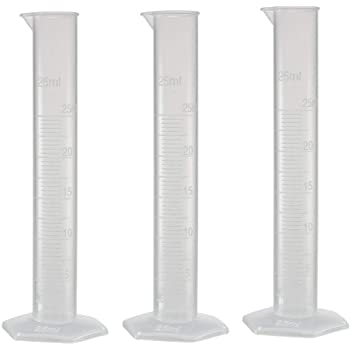
\includegraphics[width=5cm, height=5cm]{cylinders.jpg}
    \caption{Three graduated lab cylinders, corresponding to three
      eigenvectors. Prior eigenvalues not shown.}
    \label{fig:cylinder}
\end{figure}



\section{Sensor Clusterization --- Vanishing Model Error}\label{section:clusterization}
\subsection{Overview}
In this section we use Theorem \ref{thm:char} to explain how sensor
clusterization may arise in various scenarios. We first consider
sequential designs, and then simultaneous designs.



\subsection{Sequential Design}\label{subsec:clusterization sequential}
Recall the sequential optimal design scheme from section
\ref{subsec:seq vs sim} and the definition of $\obs_k$ from
\eqref{eq:def obs_k}. The way clusterization can occur in sequential
design scenario is understood by specializing thorem \ref{thm:char} to
one measurement each time. In this case $m=1$, so $k=1$, $\meas_1
\parallel \ev_1$ and $\eta_1 = 1$. As hinted in section
\ref{subsec:seq vs sim}, the posterior becomes the prior for the next
step. The eigenvectors of the new posterior are the same as for the
previous one. A new measurement will be taken in the direction of
eigenvector with smalles eigenvalue. This leads to:
\begin{align*}
  \begin{split}
    \meas_2 \parallel \ev_1  &\text{ if } \sigma^2 \lambda^{-1}_1 + 1 < \sigma^2\lambda^{-1}_2 \\
    \meas_2 \parallel \ev_2  &\text{ o.w. }
  \end{split}
\end{align*}
In the first case, we get clusterization immediately. In the second,
we consider $\meas_3$. Same reasoning leads to the conclusion that the
eigenvectors of the new prior precision are the same. The eigenvalues,
however, are $\lambda^{-1}_1 + \sigma^{-2}, \lambda^{-1}_2 +
\sigma^{-2}, \lambda_3^{-1}, \dots$. A new measurement is taken in the
direction of eigenvector of smallest precision (note that
$\lambda^{-1}_1 + \sigma^{-2} < \lambda^{-1}_2 + \sigma^{-2}$):
\begin{align*}
  \begin{split}
    \meas_3 \parallel \ev_1 &\text{ if } \sigma^2 \lambda^{-1}_1 + 1 <
    \sigma^2\lambda^{-1}_3 \\
    \meas_3 \parallel  \ev_3  &\text{ o.w. }
  \end{split}
\end{align*}
Again, the first case results in clusterization. The sequential design
proceeds in this fashion. Every $\meas_i$ is taken in the direction
some eigenvector of the prior $\fwd \prcov\fwd^*$. This eigenvector
has the smallest eigenvalue of the previous step's posterior precision
operator. If we do not encounter clusterization after $m$ such steps,
this means that measurement $\meas_k$ was taken in the direction
$\ev_k$ for $k=1,\dots,m$. Thus:
\begin{align}\label{eq:failure}
  \begin{split}
    \sigma^2\lambda_{k-1}^{-1} + 1 \geq \sigma^2\lambda_k^{-1}, \text{ for } 1\leq k \leq m
    \Longrightarrow \lambda_m^{-1} - \lambda_{m-1}^{-1} \leq \sigma^{-2}.
  \end{split}
\end{align}

But \eqref{eq:failure} implies $\{\lambda_i^{-1}\}_{i=1}^{\infty}$
grows at most linearly. In section \ref{subsec:abstract OED} we
assumed $\fwd$ is strongly smoothing, which means eigenvalues of
$(\fwd \prcov\fwd^*)^{-1}$ grow quickly. Thus, if we take $m$ large
enough, \eqref{eq:failure} will eventually fail and we will observe
sensor clusterization.


\subsection{Simultaneous Design}\label{subsec:clusterization simultaneous}
In a simultaneous design scenario, the result is not simple as in the
sequential design case. We now see that a design that exhibits
clusterization is as optimal as one that does not. Corollary
\ref{cor:same ev} tells us that we can realize any design we want
(encoded in $\{\eta_i\}$), given the trace constraint for
$\obs^*\obs$. Theorem \ref{thm:char} tells us that for D-optimality,
we only need to make the posterior flat where we take measurements
(recall figure \ref{fig:optimal vs not}). We are left with the freedom
of assigning any part of $\eta_i$ to any measurement $\meas_j$. Two
possible assignments for the same problem are illustrated in figure
\ref{fig:clusterization}. The first exhibits clusterization and second
does not. It is important to note that neither arises as a result of
some numerical optimization scheme. Both designs are give the same
design criterion $\tar$, because their posteriors are identical. By
Theorem \ref{thm:char}, both are (possible) maximizers to the same
D-optimal design problem. One exhibits clusterization, and one does
not. It is possible that a real-life problem is more restricted than
the model we consider here. Exactly in what way this happens is not
clear and should be the subject of further research.


\begin{figure}
  \begin{tikzpicture}[scale=0.85]
    \begin{axis}[
        ybar stacked,
        ymin=0,
        ymax=4,
        xtick=data,
        legend style={cells={anchor=east}, legend pos=north west, legend columns=-1},
        reverse legend=false, % set to false to get correct display, but I'd like to have this true
        xticklabels from table={\clusterization}{Label},
        xticklabel style={text width=2cm,align=center},
        legend plot pos=right,
        ylabel=precision --- prior and posterior,
        xlabel=eigenvector $i$,
      ]
    
      
      \addplot [fill=green!80]  table [y=prior, meta=Label, x expr=\coordindex] {\clusterization};
      \addplot [fill=blue!60]   table [y=$o_1$, meta=Label, x expr=\coordindex] {\clusterization};
      \addplot [fill=red!60]    table [y=$o_2$, meta=Label, x expr=\coordindex] {\clusterization};
      \addplot [fill=black!60]  table [y=$o_3$, meta=Label, x expr=\coordindex] {\clusterization};
      \addplot [fill=orange!60] table [y=$o_4$, meta=Label, x expr=\coordindex] {\clusterization};
      \addplot [fill=cyan!60]   table [y=$o_5$, meta=Label, x expr=\coordindex] {\clusterization};
      \addplot [fill=purple!60] table [y=$o_6$, meta=Label, x expr=\coordindex] {\clusterization};

      
      \addlegendentry{prior}
      \addlegendentry{$o_1$}
      \addlegendentry{$o_2$}
      \addlegendentry{$o_3$}
      \addlegendentry{$o_4$}
      \addlegendentry{$o_5$}
      \addlegendentry{$o_6$}   
    \end{axis}
  \end{tikzpicture}
  \qquad
  \begin{tikzpicture}[scale=0.85]
    \begin{axis}[
        ybar stacked,
        ymin=0,
        ymax=4,
        xtick=data,
        legend style={cells={anchor=east}, legend pos=north west, legend columns=-1},
        reverse legend=false, % set to false to get correct display, but I'd like to have this true
        xticklabels from table={\noclusterization}{Label},
        xticklabel style={text width=2cm,align=center},
        legend plot pos=right,
        ylabel=precision --- prior and posterior,
        xlabel=eigenvector $i$,
      ]
    
      
      \addplot [fill=green!80]  table [y=prior, meta=Label, x expr=\coordindex] {\noclusterization};
      \addplot [fill=blue!60]   table [y=$o_1$, meta=Label, x expr=\coordindex] {\noclusterization};
      \addplot [fill=red!60]    table [y=$o_2$, meta=Label, x expr=\coordindex] {\noclusterization};
      \addplot [fill=black!60]  table [y=$o_3$, meta=Label, x expr=\coordindex] {\noclusterization};
      \addplot [fill=orange!60] table [y=$o_4$, meta=Label, x expr=\coordindex] {\noclusterization};
      \addplot [fill=cyan!60]   table [y=$o_5$, meta=Label, x expr=\coordindex] {\noclusterization};
      \addplot [fill=purple!60] table [y=$o_6$, meta=Label, x expr=\coordindex] {\noclusterization};

      
      \addlegendentry{prior}
      \addlegendentry{$o_1$}
      \addlegendentry{$o_2$}
      \addlegendentry{$o_3$}
      \addlegendentry{$o_4$}
      \addlegendentry{$o_5$}
      \addlegendentry{$o_6$}   
    \end{axis}
  \end{tikzpicture}
  \caption{Clusterization (left) and non-clusterization (right) in
    simultaneous D-optimal designs. Posterior precision per
    eigenvector after taking measurements $\meas_i$ is plotted. Both
    designs are identical for all practical matters --- their
    posteriors are identical. In the left panel we see how an optimal
    design is achieved with repeated measurements. $\meas_2 = \meas_3$
    and $\meas_5 = \meas_6$. This is not necessary though, as can be
    seen in the right panel. Both designs achieve the same levels of
    uncertainty. The left exhibits clusterization. The right does not.}
  \label{fig:clusterization}
\end{figure}







%%%%%%%%%%%%%%%%%%%%%%%%%%%%%%%%%%%%%%%%%%%%%%%%%%%%%%%%%%%%%%%%
%% SECTION Analysis of Optimal Designs --- Non-Vanishing Model Error
%%%%%%%%%%%%%%%%%%%%%%%%%%%%%%%%%%%%%%%%%%%%%%%%%%%%%%%%%%%%%%%%
\section{Analysis of D-Optimal Designs --- Non-Vanishing Model Error}\label{section:non vanishing}
In this section we show the effect model error has on the
clusterization phenomenon. We will see that if $\modcov \neq 0$
clustering will not occur. This is contrary to the previous case of
vanishing model error.

Corollary \ref{cor:same meas} below is proved in the appendix. Denote
$\obs = (\meas_1,\dots,\meas_m)^t$ and $\obsm :=
(\meas_1,\dots,\meas_{m-1})^t$. Denote $\Sigmam := \Sigma (\obsm)$ and
$\postcovm$ the posterior covariance that arises when we use $\obsm$.
\begin{restatable*}{corollary}{samemeas}\label{cor:same meas}
  If $\meas_m = \meas_j$ for some $1 \leq j \leq m-1$, then
  \begin{equation*}
    \tar(\obs) - \tar(\obsm) =
    \log \left ( 1 + \frac{\sigma^2
      \langle \fwd \postcovm \fwd^* \obsm^* \Sigmam^{-1} e_j,
      \obsm^* \Sigmam^{-1}e_j \rangle
    }{
      2 - \sigma^2 e_j^t\Sigmam^{-1}e_j 
    }       
    \right ).
  \end{equation*}
\end{restatable*}
Recall from \eqref{eq:Sigma} that $\Sigma(\obs) = \obs \modcov \obs^*
+ \sigma^2I$. Then

$$
\lim_{\sigma^2 \to 0} \tar(\obs) -\tar(\obsm) = 0
$$

Hence no increase in the design criterion is achieved by taking a
repeated measurement (in the limit $\sigma^2 \to 0$). This is clearly
sub-optimal and $\obsm$ cannot be a D-optimal design. Thus, for small
measurement error levels, the clusterization effect will be mitigated
by the presence of a non-zero model error. Since the design criterion
is not defined for $\sigma^2 = 0$ and identical measurements, we
cannot make a statement regarding $\sigma^2 = 0$, except in the
limiting sense described above.


\section{Acknowledgements}
This study is a part of my PhD thesis. Most of it was written under
the instruction of Prof. Georg Stadler in New York University's
Courant Institute. I would like to thank him for his great
mentorship. This work was supported by The Raymond and Beverly Sackler
Post-Doctoral Scholarship.

\appendix
\section{General Lemmas}

The following lemma is generalized from \cite[Chapter 9, Theorem 4, pp. 127]{Lax97}
\lax
\begin{proof}
  Consider a differentiable operator-valued function $X(t)$ such that
  $X(0) = 0$ and $X(t)$ is positive, self-adjoint and trace-class for
  every $t\in \R$. We denote the eigenvalues of this operator by
  $\lambda_k(X(t))$ and sometimes drop the dependence on $X(t)$, so
  $\lambda_k = \lambda_k(X(t))$.  Then $\det (I+X(t)) =
  \prod_{k=1}^{\infty} (1+\lambda_k) < \infty$ where the bound holds
  by the arguments given in \cite{AlexanderianGloorGhattas14}. The
  full derivative is
  \begin{align*}
    \frac{\der \det (I+X(t))}{\der t} 
    % 
    % 
    % 
    &= \sum_{k=1}^{\infty} 
    \frac{\partial \det (I+X(s))}{\partial (1+\lambda_k)}\Big |_{s=t}
    \frac{\der (1+\lambda_k)}{\der t} \\
    % 
    %
    %
    &= \sum_{k=1}^{\infty} \frac{\partial \prod_{l=1}^{\infty}
      (1+\lambda_l(s))}{\partial (1+\lambda_k)}\Big |_{s=t}
    \frac{\der (1+\lambda_k)}{\der t} \\
    %
    %
    %
    &= \sum_{k=1}^{\infty} \prod_{l=1, l\neq k}^{\infty}
      (1+\lambda_l(s)) \frac{\partial (1+\lambda_k(s))}{\partial (1+\lambda_k)}\Big |_{s=t}
    \frac{\der (1+\lambda_k)}{\der t} \\
    %
    %
    %    
    &= \sum_{k=1}^{\infty} \frac{\prod_{l=1}^{\infty}
      (1+\lambda_l(s))}{(1+\lambda_k)}\Big |_{s=t}
    \dot{\lambda_k}(X(t)) \\
    % 
    % 
    % 
    &= \sum_{k=1}^{\infty} \frac{\det (I+X(t))}{1 +\lambda_k} \dot{\lambda_k}(X(t)).
  \end{align*}
  The assumption $X(0) = 0$ means $\lambda_k(X(0)) = 0,\ \forall k \geq 1$. Thus:
  \begin{align*}
    \frac{\der (I+\det X(t))}{\der t}\Big |_{t=0} 
    = \sum_{k=1}^{\infty} \dot{\lambda_k}(X(0)) 
    = \frac{\der }{\der t}\tr{X(0)}
    = \tr{\dot{X}(0)},
  \end{align*}
  where the second equality follows by monotone convergence. 
  Let $Y(t)$ a trace-class self-adjoint operator such that 
  $I+Y(t)$ is invertible.
  Define $X(t)$ via $I+X(t) = (I+Y(0))^{-1/2} (I+Y(t)) (I+Y(0))^{-1/2}$. 
  We show $X(t)$ satisfies the conditions above. It is trace-class:
  \begin{align*}
    \tr{X(t)} = \tr{(I+Y(0))^{-1} (I+Y(t)) - I}
    \leq \tr{I+Y(t) - I}< \infty,
  \end{align*}
  since $Y(t)$ is trace-class. It is also clear that
  $X(0) = 0$ and $X(t)$ is self-adjoint.
  $I+Y(t) = (I+Y(0))^{1/2}(I+X(t))(I+Y(0))^{1/2}$, so
  \begin{align*}
    \frac{\der \det (I+Y(t))}{\der t}|_{t=0} 
    &= \det (I+Y(0))\frac{\der \det (I+X(t))}{\der t}\Big |_{t=0} \\
    % 
    % 
    % 
    &= \det (I+Y(0)) \tr{\dot{X}(0)} \\
    % 
    % 
    % 
    &= \det (I+Y(0)) \tr{(I+Y(0))^{-1} \dot{Y}(0)}.
  \end{align*}
  Consequently, by the one-variable chain rule:
  \begin{align*}
    \frac{\der \log \det (I+Y(t))}{\der t}\Big |_{t=0} &=
    % 
    % 
    % 
    \frac{1}{\det (I+Y(0))}\frac{\der \det (I+Y(t))}{\der t}\Big |_{t=0} \\ 
    % 
    % 
    % 
    &= \tr{ (I+Y(t))^{-1} \dot{Y}(t)} \big |_{t=0}.
  \end{align*}
  There is nothing special about $t_0 = 0$ --- we could have chosen
  any other $t_0$ instead. Thus, the relation holds for all $t$.
\end{proof}


\begin{lemma}[Matrix Determinant Lemma in Hilbert Spaces]\label{lemma:MDL}
  Let $\hil$ a separable Hilbert space, $u,v\in \hil$ and $A: \hil \to
  \hil$ an invertible linear operator such that $\tr{A-I} <
  \infty$. Then $\det A$ and $\det A + uv^*$ are well defined and
  \begin{equation*}
    \det (A + uv^*) = (1 + \langle A^{-1} u, v \rangle ) \det A,
  \end{equation*}
  where $(A + uv^*)w := Aw + \langle v,w \rangle u$.
\end{lemma}
\begin{proof}
  In this proof we rely on definitions and results from
  \cite{Simon77}. First, consider $B := I + xy^*$ for some $x,y \in
  \hil$. We construct an eigenbasis for $B$ and use that to show $\det
  B = 1 + \langle x, y \rangle$. First let $x_1 := x$.  Now, if $x
  \parallel y$, take $\{x_n \}_{n=2}^{\infty}$ an orthogonal basis for
  $span\{x_1\} ^{\perp}$. If, on the other hand, $x \nparallel y$, let
  \begin{equation*}
    x_2 := x - \frac{ \langle x, y\rangle}{\|y\|^2}y
  \end{equation*}
  and it is easy to verify that $x_2 \perp y$ and $span \{x,y\} = span
  \{x_1,x_2\}$. Take $\{x_n \}_{n=3}^{\infty}$ an orthogonal basis for
  $span\{x_1,x_2\} ^{\perp}$. In both cases,
  \begin{equation*}
    B x_n =
    \begin{cases}
      (1 + \langle x, y \rangle) x_n & n = 1 \\
      x_n                            & n \neq 1,
    \end{cases}
  \end{equation*}
  and so $\det B = 1 + \langle x, y \rangle$.
  
  It is easy to verify that $uv^*$ is trace-class and since $\tr{A-I}
  < \infty$, also $\tr{A + uv^* - I} < \infty$ (sum of two trace-class
  operators is trace-class). Thus $\det A$ and $\det (A+uv^*)$ are
  well defined. Let $x:=A^{-1}u$ and $y := v$:
  \begin{equation*}
    \det (A + uv^*) = \det A \ \det(I+A^{-1}uv^*) =
    (1 + \langle A^{-1}u, v \rangle) \det A .
  \end{equation*}
\end{proof}


\free
\begin{proof}
  Let us diagonalize $M$, so that $M = U D U^t$ with $D =
  \diag(d_1,\dots,d_k)$ and $U \in \R^{k \times k }$ orthogonal. Let
  $S \in \R^{k \times m}$ with $S_{ii} = \sqrt{d_{i}}$ and zeros
  otherwise. Define $A:= U S V^t$, where $V \in \R^{m \times m}$ is
  orthogonal and will be further restricted later. Then $AA^t = U
  SV^tVS^t U^t = UDU^t$, so $AA^t$ has the required eigenvalues and
  eigenvectors by construction. If we can choose $V$ such that $A$
  also satisfies the unit norm constraints we are done. These
  constraints are, for $j=1,\dots,m$:
  \begin{equation}\label{eq:V constraints}
   1 = [A^tA]_{jj} = [V S^tS V^t]_{jj},
  \end{equation}
  and we can expect to do this since we assumed $\ttr D = m$.

  Define $C = S^tS - I \in \R^{m \times m}$. Note that $\ttr C = 0$ and
  $C$ is diagonal with non-zero entries $d_i-1,i=1,\dots,k$. It suffices
  to find $V$ orthogonal such that $V C V^t$ has zero diagonal. We
  construct such $V$ by sequentially inserting zeros in the diagonal
  and not destroying zeros we already introduced, starting from the
  last diagonal entry and moving to the first. Since $c_{mm} \neq 0$ ,
  let $p < m$ such that $c_{pp}c_{mm} < 0$ (such $p$ exists because
  the trace is zero) and let $\theta \in (0,\pi)$. Define a Givens
  rotation $R^{(m)} \in \R^{m \times m}$ by
  \begin{equation*}
    r^{(m)}_{ab} :=
    \begin{cases}
      1 & a = b \neq p \text{ or } a = b \neq m \\
      \cos \theta & a = b = p  \\
     -\sin \theta & a = p, b = m\\
      \cos \theta & a = b = m \\
      \sin \theta & a = m, b = p \\ 
      0 & o.w
    \end{cases}
  \end{equation*}
  Note that conjugating a matrix by $R^{(m)}$ changes only its $m$ and
  $p$ rows and columns. We want to choose $\theta$ such that
  \begin{equation}\label{eq:mm}
    0 = [R^{(m)} C (R^{(m)})^t]_{mm} = \cos^2 \theta c_{mm} + 2\cos \theta \sin
    \theta c_{mp} + \sin^2\theta c_{pp},
  \end{equation}
  and it suffices to choose $\theta$ such that
  \begin{equation*}
    c_{mm} \cot^2 \theta + 2 c_{mp} \cot \theta + c_{pp} = 0.
  \end{equation*}
  This quadratic in $\cot\theta$ has a real solution, since
  $c_{pp}c_{mm} < 0$ by assumption and we can find $\theta \in
  (0,\pi)$ such that \eqref{eq:mm} is satisfied. We continue to find
  $R^{(m-1)}$ that leaves row and column $m$ unchanged and
  continue introducing zeros to the diagonal. The assumption $\ttr D =
  m \Rightarrow \ttr C = 0$ guarantees we can do that. Taking $V:=
  R^{(1)} R^{(2)} \dots R^{(m-1)}R^{(m)}$ completes the proof.
\end{proof}


\simdiag
\begin{proof}
  First, enumerate the eigenvalues of $C + \sum_{j=1}^m
  \func_j\func_j^*$ as $\xi_1,\dots,\xi_\ell$. Denote the
  indices of the eigenvectors corresponding to $\xi_i$
  \begin{equation*}
    S_i := \{ 1 \leq k \leq m | (C + \sum_{j=1}^m \func_j\func_j^* )\func_k = \xi_i \func_k \}.
  \end{equation*}
  Define further
  \begin{equation*}
    A_i := \sum_{k \in S_i} \func_k \func_k^*,
  \end{equation*}
  which is self-adjoint. Two observations are in order. First,
  $\sum_{j=1}^m \func_j\func_j^* = \sum_{i=1}^\ell A_i$. Second, $A_i
  \func_k = 0$ if $k\not \in S_i$, since eigenvectors of different
  eigenvalue are orthogonal. For $k \in S_i$
  \begin{equation}\label{eq:on vi}
    \xi_i \func_k = (C + \sum_{j=1}^m \func_j \func_j^* ) \func_k = (C + A_i) \func_k.
  \end{equation}
  Let $V_i := span \{\func_k \}_{k\in S_i}$. Observe that $V_i$ is
  invariant under $A_i$, by definition, and under $C$, by \eqref{eq:on
    vi}. Using \eqref{eq:on vi} again, we conclude that on $V_i$, $A_i
  = \xi_iI - C$. This immediately implies $A_i$ and $C$ have the
  same eigenvectors on $V_i$. This holds for every $1 \leq i \leq
  \ell$ and we conclude that $C$ and $A$ have the same eigenvectors.
\end{proof}


\section{Specific Lemmas}

%%%%%%%%%%%%%%%%%%%%%%%%%%%%%%%%%%%%%%%%%%%%%%%%%%%%%%%%%%%%%%%%%%%%%%%%%
\begin{lemma}\label{lemma:twice woodbury}
  Assume $\fwd \prcov \fwd^*$ is invertible. Then
\begin{align*}
  \begin{split}
    \fwd( \prcov^{-1} + \sigma^{-2}  \fwd^* \obs^* \obs \fwd )^{-1} \fwd^* 
    %
    %
    = \left ( (\fwd\prcov\fwd^*)^{-1} + \sigma^{-2}  \obs^* \obs \right )^{-1},
  \end{split}
\end{align*}  
\end{lemma}
\begin{proof}
  The proof is boring and amounts to using Woodbury's matrix identity
  twice and a regularization trick. The standard proof for this
  identity works in infinite dimensions, as long as all terms are well
  defined. Unfortunately, $\obs^*\obs$ is not invertible, so we force
  it to be. Throughout, we let $X := \fwd\prcov \fwd^*$ and $Y_{\eps}
  := \obs^*\obs + \eps I$, for some small $\eps > 0$. Note that now
  $Y_{\eps}$ is invertible. Recall Woodbury's matrix identity:
  $$
  (A + UCV)^{-1} = A^{-1} + A^{-1}U(C^{-1} + VA^{-1}U)^{-1}VA^{-1}.
  $$

  Taking $A := \prcov^{-1}, U := \fwd^*, V := \fwd$ and $C :=
  \sigma^{-2} (\obs^*\obs+\eps I)$ we get:
  \begin{align*}
    \begin{split}
      \fwd( \prcov^{-1} + \sigma^{-2}  \fwd^* (\obs^* \obs +\eps I) \fwd )^{-1}\fwd^* &=
      \fwd ( \prcov - \prcov \fwd^* ( \sigma^2(\obs^*\obs + \eps I)^{-1} + \fwd \prcov \fwd^* )^{-1} \fwd \prcov ) \fwd^* \\
      %
      %
      &= X - X(\sigma^2Y_{\eps}^{-1} + X)^{-1}X
    \end{split}
  \end{align*}
  Note that $X + \sigma^2 Y_{\eps}^{-1}$ is invertible, as the sum of
  a two positive definite operators. Now, taking $A := X^{-1}, C :=
  \sigma^2Y_{\eps}^{-1}, U := I$ and $V := I$ and using Wodbury's matrix
  identity in reverse order:
  \begin{align*}
    \begin{split}
      X - X(\sigma^2Y_{\eps}^{-1} + X)^{-1}X &= (X^{-1} + \sigma^{-2}Y_{\eps})^{-1} \\
      %
      %
      %
      &= (\fwd \prcov \fwd^* + \sigma^{-2} (\obs^*\obs + \eps I))^{-1}.
    \end{split}
  \end{align*}

  We conclude that $\forall \eps > 0$
  \begin{align*}
    \begin{split}
      \fwd( \prcov^{-1} + \sigma^{-2}  \fwd^* (\obs^* \obs +\eps I) \fwd )^{-1}\fwd^* 
     &= (\fwd \prcov \fwd^* + \sigma^{-2} (\obs^*\obs + \eps I))^{-1}.
    \end{split}
  \end{align*}
  Letting $\eps \to 0$ completes the proof.
\end{proof}



%%%%%%%%%%%%%%%%%%%%%%%%%%%%%%%%%%%%%%%%%%%%%%%%%%%%%%%%%%%%%%%%%%%%%%%%%
\begin{lemma}[Increase due to a Measurement]\label{lemma:design increase}
  Let $\obs = (\meas_1,\dots,\meas_m)^t$ and $\obsm := (\meas_1,\dots,\meas_{m-1})^t$. Then
  \begin{align*}
    \tar( \obs ) - \tar (\obsm ) &=
    \frac12 \log \left ( 1 + \frac{
      \langle \fwd \postcovm \fwd^* (\obsm^* \Sigmam^{-1} \modcov - I ) \meas_m,
      (\obsm^* \Sigmam^{-1} \modcov - I ) \meas_m \rangle
    }{
      \sigma^2 + \meas_m \modcov \meas_m - \meas_m \modcov \obsm^* \Sigmam^{-1} \obsm \modcov \meas_m 
    }       
    \right ).
  \end{align*}
\end{lemma}
\begin{proof}
  We use the Schur complement to write one inverse in terms of the other and
  introduce notations to make the derivation cleaner. Note that we think of
  $\obsm$ and $\obsm^*$ as column and row vectors (respectively).
  \begin{align*}
    \Sigma( \obs ) &= \Sigma = 
    \begin{bmatrix}
      \Sigma (\obsm )           & \obsm \modcov \meas_m \\
      \meas_m \modcov \obsm^*   & \sigma^2 + \meas_m \modcov \meas_m
    \end{bmatrix}
    =
    \begin{bmatrix}
      \Sigmam   & w \\
      w^t       & c
    \end{bmatrix}\\
    %
    %
    %
    \Sigma^{-1} &=
    \begin{bmatrix}
      \Sigmam^{-1} + \Sigmam^{-1} w ( c - w^t \Sigmam^{-1} w)^{-1} w^t \Sigmam^{-1} & - \Sigmam^{-1} w ( c - w^t \Sigmam^{-1} w)^{-1} \\
      -( c - w^t \Sigmam^{-1} w)^{-1} w^t \Sigmam^{-1}                            &  ( c - w^t \Sigmam^{-1} w)^{-1}
    \end{bmatrix} \\
    &=
    \begin{bmatrix}
      \Sigmam^{-1} & 0 \\
      0           & 0 
    \end{bmatrix}
    + (c -w^t \Sigmam^{-1} w )^{-1}
    \begin{bmatrix}
      \Sigmam^{-1} w \\
      -1
    \end{bmatrix}
    \begin{bmatrix}
      w^t \Sigmam^{-1} & -1 
    \end{bmatrix}
  \end{align*}
  %
  Further, define
  %
  \begin{align*}
    \M (\obs ):&= \prcov^{\frac12}\fwd^* \obs^* \Sigma^{-1} \obs \fwd
    \prcov^{\frac12}    
  \end{align*}
  %
  and note that, using our understanding of what is a column vector and
  what is a row vector:
  %
  \begin{align*}
    \M(\obs) &= \prcov^{1/2} \fwd^* \obs^* \Sigma^{-1} \obs \fwd \prcov^{1/2} \\
    %
    %
    %
    &= \prcov^{1/2} \fwd^* \obs^* \left \{
    \begin{bmatrix}
      \Sigmam^{-1} & 0 \\
      0           & 0 
    \end{bmatrix}
    + (c -w^t \Sigmam^{-1} w )^{-1}
    \begin{bmatrix}
      \Sigmam^{-1} w \\
      -1
    \end{bmatrix}
    \begin{bmatrix}
      w^t \Sigmam^{-1} & -1 
    \end{bmatrix} 
    \right \} \obs \fwd \prcov^{1/2} \\
    %
    %
    %
    &= \M (\obsm) + (c -w^t \Sigmam^{-1} w )^{-1}
    \prcov^{1/2} \fwd^* \obs^*
    \begin{bmatrix}
      \Sigmam^{-1} w \\
      -1
    \end{bmatrix}
    \begin{bmatrix}
      w^t \Sigmam^{-1} & -1 
    \end{bmatrix} 
    \obs \fwd \prcov^{1/2}
  \end{align*}
  %
  Now, denote:
  %
  \begin{align}\label{eq:u}
    \begin{split}
      u :&= (c -w^t \Sigmam^{-1} w )^{-1/2}
      \prcov^{1/2} \fwd^* \obs^* 
      \begin{bmatrix}
        \Sigmam^{-1} w \\
        -1 
      \end{bmatrix} \\
      %
      %
      %
      & = (c -w^t \Sigmam^{-1} w )^{-1/2} ( \prcov^{1/2}\fwd^* \obsm^* \Sigmam^{-1} \obsm  \modcov \meas_m - \prcov^{1/2} \fwd^* \meas_m )\\
      %
      %
      %
      u^* :&=  (c -w^t \Sigmam^{-1} w )^{-1/2} (\meas_m \modcov \obsm^* \Sigmam^{-1} \obsm \fwd \prcov^{1/2} - \meas_m \fwd \prcov^{1/2} ),
    \end{split}
  \end{align}
  %
  so that
  %
  \begin{equation}\label{eq:M plus I}
    I + \M( \obs ) = I + \M (\obsm ) + uu^*.
  \end{equation}
  %
  Note that
  \begin{equation}\label{eq:M postcov}
    \prcov^{1/2} \left (I + \M( \obsm ) \right )^{-1} \prcov^{1/2} = \postcovm.
  \end{equation}
  The increase in the design criterion gained by including $\meas_m$
  in the design is found by using Lemma \ref{lemma:MDL} the above
  results:
  %
  \begin{align*}
    \tar( \obs ) - \tar( \obsm )
    %
    %
    %
    &= \frac12 \log \det \Big ( I + \M ( \obs ) \Big ) / \det \Big ( I + \M (\obsm) \Big ) \\
    %
    %
    %
    &= \frac12  \log \det \left ( I + \M(\obsm) + uu^* \right ) / \det \Big ( I + \M (\obsm) \Big ) \\
    %
    %
    %
    &= \frac12 \log \left ( 1 + \left \langle \left ( I+\M(\obsm) \right )^{-1} u, u  \right \rangle \right ).
  \end{align*}
  Using \eqref{eq:u}:
  \begin{align*}
    &\left \langle \left (I+\M (\obsm)\right )^{-1}u, u \right \rangle\\
    &= \frac{
      \langle \fwd \postcovm \fwd^* (\obsm^* \Sigmam^{-1} \obsm \modcov - I ) \meas_m,
      (\obsm^* \Sigmam^{-1} \obsm \modcov - I ) \meas_m \rangle
    }{
      c- w^t \Sigmam^{-1} w
    }\\
    %
    %
    %
    &= 
    \frac{
      \langle \fwd \postcovm \fwd^* (\obsm^* \Sigmam^{-1} \obsm \modcov - I ) \meas_m,
      (\obsm^* \Sigmam^{-1} \obsm \modcov - I ) \meas_m \rangle
    }{
      \sigma^2 + \meas_m \modcov \meas_m - \meas_m \modcov \obsm^* \Sigmam^{-1} \obsm \modcov \meas_m 
    }
  \end{align*}
  and the conclusion follows.
\end{proof}

Lemma \ref{lemma:design increase} implies the following two corollaries.
\begin{corollary}[Gain for No Model Error]\label{cor:zero mod err}
  If $\modcov = 0$, then
  \begin{equation*}
    \tar( \obs ) - \tar (\obsm )
    = -\frac12 \log (1 - \sigma^{-2} \langle \fwd \postcov \fwd^* \meas_m, \meas_m \rangle ).
  \end{equation*}
\end{corollary}
\begin{proof}
  Note that this is not immediate by substituting $\modcov = 0$ in the
  conclusion of Lemma \ref{lemma:design increase}, since we make a
  claim for $\postcov$, and not $\postcovm$. Let us first review
  \eqref{eq:u} and note that since $\modcov = 0$ the covariance
  $\Sigmam = \sigma^2I_{m-1}$ and $w = 0$, so $c - w^t\Sigmam^{-1}w =
  \sigma^2$:
  \begin{align*}
    u :&=-\sigma^{-1}\prcov^{1/2} \fwd^* \meas_m\\
    %
    %
    u^* :&= -\sigma^{-1} \meas_m \fwd \prcov^{1/2}.
  \end{align*}
  From \eqref{eq:M plus I}:
  \begin{equation*}
    I + \M(\obsm) = I +\M(\obs) - uu^*,
  \end{equation*}
  and thus:
  \begin{equation*}
    \left \langle \left ( I +\M(\obs) \right )^{-1} u, u \right \rangle
    = \sigma^{-2} \langle \fwd \postcov \fwd^* \meas_m, \meas_m \rangle.
  \end{equation*}
  Analogously to \eqref{eq:M postcov} we note that
  \begin{equation*}
    \prcov^{1/2} \left ( I + \M(\obs) \right )^{-1} \prcov^{1/2} = \postcov.
  \end{equation*}
  Using Lemma \ref{lemma:MDL} we conclude
  \begin{align*}
    \tar( \obs ) - \tar( \obs )
    &= \frac12 \log \det \left (I +\M(\obs) \right ) / \det \left (I + \M(\obsm) \right ) \\
    %
    %
    %
    &= \frac12 \log \det \left (I +\M(\obs) \right ) / \det \left (I + \M(\obs) - uu^* \right ) \\
    %
    %
    %
    &=-\frac12 \log (1 - \langle (I+\M(\obs))^{-1}u, u \rangle \\
    %
    %
    %
    &= -\frac12 \log (1 - \sigma^{-2} \langle \fwd \postcov \fwd^* \meas_m, \meas_m \rangle ).
  \end{align*}
\end{proof}

\samemeas
\begin{proof} \label{cor:same meas proof}
  Denote $A:= \obs \modcov \obs^*$ and $v_j$ the $j$th column of $A$.
  Note that $v_j = \obsm \modcov \meas_m$, since $(\obsm \modcov
  \obsm^*)_{ij} = \meas_i(\modcov \meas_j)$, as explained in
  \eqref{eq:modcov explained}. One can now verify that
  \begin{equation}\label{eq:observation}
    \Sigmam^{-1} \obsm \modcov \meas_m = \Sigmam^{-1}v_j = (A +\sigma^2I_{m-1})^{-1} v_j =
    e_j -\sigma^2 \Sigmam^{-1}e_j.
  \end{equation}
  %
  Using \eqref{eq:observation}:
  \begin{align}\label{eq:denominator}
    \begin{split}
      \meas_m \modcov \obsm^* \Sigmam^{-1} \obsm \modcov \meas_m
      &= \meas_m \modcov \obsm^* ( e^j - \sigma^2 \Sigmam^{-1} e_j )\\
      %
      %
      %
      &= \meas_m \modcov \meas_j - \sigma^2 \meas_m \modcov \obsm^* \Sigmam^{-1}e_j \\
      %
      %
      %
      &= \meas_m \modcov \meas_j -\sigma^2 (e_j - \sigma^2 \Sigmam^{-1}e_j)^t e_j \\
      %
      %
      %
      &= \meas_m \modcov \meas_m -\sigma^2 + \sigma^4 e_j^t\Sigmam^{-1}e_j.
    \end{split}
  \end{align}
  We use \eqref{eq:observation} to simplify the terms in the enumerator of
  the conclusion of Lemma \ref{lemma:design increase}:
  \begin{align}\label{eq:enumerator}
    \begin{split}
      (\obsm^* \Sigmam^{-1} \obsm \modcov - I ) \meas_m
      &= \obsm^* \Sigmam^{-1} \obsm \modcov \meas_m - \meas_m \\
      %
      %
      %
      &= \obsm^* (e_j - \sigma^2 \Sigmam^{-1} e_j) -\meas_j \\ 
      %
      %
      %
      &= -\sigma^2 \obsm^* \Sigma^{-1}e_j. 
    \end{split}
  \end{align}
  %
  Substitute \eqref{eq:enumerator} and \eqref{eq:denominator} to
  the enumerator and denominator (respectively) of the conclusion of
  Lemma \ref{lemma:design increase}:
  %
  \begin{align*}
    \tar( \obs ) - \tar (\obsm ) &=
    \log \left ( 1 + \frac{
      \langle \fwd \postcovm \fwd^* (\obsm^* \Sigmam^{-1} \modcov - I ) \meas_m,
      (\obsm^* \Sigmam^{-1} \modcov - I ) \meas_m \rangle
    }{
      \sigma^2 + \meas_m \modcov \meas_m - \meas_m \modcov \obsm^* \Sigmam^{-1} \obsm \modcov \meas_m 
    }       
    \right ) \\
    %
    %
    %
    &= \log \left ( 1 + \frac{\sigma^4
      \langle \fwd \postcovm \fwd^* \obsm^* \Sigmam^{-1} e_j,
      \obsm^* \Sigmam^{-1}e_j \rangle
    }{
      2\sigma^2 - \sigma^4 e_j^t\Sigmam^{-1}e_j 
    }       
    \right ) \\
    %
    %
    %
    &= \log \left ( 1 + \frac{\sigma^2
      \langle \fwd \postcovm \fwd^* \obsm^* \Sigmam^{-1} e_j,
      \obsm^* \Sigmam^{-1}e_j \rangle
    }{
      2 - \sigma^2 e_j^t\Sigmam^{-1}e_j 
    }       
    \right ).
  \end{align*}
\end{proof}


\begin{lemma}[Auxilliary Calculations]\label{lemma:aux calc}
  Let $T(\obs) := \obs^* \Sigma^{-1}(\obs)\obs$, with $\Sigma(\obs)$
  defined as in \eqref{eq:Sigma}. Then:
  \begin{align*}
    \delta T(\obs)V &= V^* \Sigma^{-1} \obs 
    - \obs^*\Sigma^{-1} V\modcov \obs^* \Sigma^{-1}\obs \\
    &\ \ \ - \obs^* \Sigma^{-1} \obs \modcov V^* \Sigma^{-1}\obs
    + \obs^* \Sigma^{-1} V.
  \end{align*}
\end{lemma}

\begin{proof}
  We need a few supplementary calculations. First:
  \begin{align}\label{eq:der sig}
    \begin{split}
      \frac{\der}{\der \tau} \Big |_{\tau=0} \Sigma( \obs + \tau V )
      &= \frac{\der}{\der \tau} \Big |_{\tau=0} 
      (\obs + \tau V ) \modcov (\obs + \tau V )^*  + \sigma^2I\\
      % 
      % 
      % 
      &= V \modcov \obs^* + \obs \modcov V^*.
    \end{split}
  \end{align}
  By the standard trick for the derivative of an operator: 
  \begin{align*}
    0 &= \frac{\der}{\der \tau} \Big |_{\tau=0} I \\
    % 
    % 
    % 
    &= \frac{\der}{\der \tau} \Big |_{\tau=0}
    \left (\Sigma(\obs+\tau V)^{-1} \Sigma(\obs+\tau V) \right ) \\
    % 
    % 
    % 
    &= \frac{\der \Sigma(\obs+\tau V)^{-1}}{\der \tau} \Big |_{\tau=0} \Sigma+
    \Sigma^{-1} \frac{\der \Sigma(\obs+\tau V)}{\der \tau} \Big |_{\tau=0}\\  
    %
    %
    %
    &= \frac{\der \Sigma(\obs+\tau V)^{-1}}{\der \tau} \Big |_{\tau=0} \Sigma+
    \Sigma^{-1} (V\modcov \obs^* + \obs \modcov V^*) 
    \text{, by \eqref{eq:der sig}. }
  \end{align*}
  Now we can write the variation of $\Sigma^{-1}$:
  \begin{align}\label{eq:der sig inv}
    \frac{\der \Sigma(\obs+\tau V)^{-1}}{\der \tau} \Big |_{\tau=0}  
      &= -\Sigma^{-1} (V \modcov \obs^* + \obs \modcov V^*) \Sigma^{-1}.
    \end{align}
  % 
  Finally, we can do the calculation we need to. By Leibnitz (product) rule
  and \eqref{eq:der sig inv}:
  % 
  \begin{align*}
    \delta T(\obs) V 
    &= \frac{\der T(\obs + \tau V)}{\der \tau} \Big |_{\tau=0} \\
    %
    %
    %
    &= V^* \Sigma^{-1} \obs 
    - \obs^*\Sigma^{-1} V\modcov \obs^* \Sigma^{-1}\obs \\
    &\ \ \ - \obs^* \Sigma^{-1} \obs \modcov V^* \Sigma^{-1}\obs
    + \obs^* \Sigma^{-1} V,
  \end{align*}
  as required.
\end{proof}

\biggerbetter
\begin{proof} 
  Fix an arbitrary $j=1,\dots,m$ and take $V:= e_j e_j^t \obs$. We see
  that for $u \in \hilo$
  \begin{equation*}
    Vu = e_je_j^t (\meas_1(u),\dots,\meas_m(u) )^t = e_j \meas_j(u)
    = (0,\dots,0,\meas_j(u),0,\dots,0)^t.
  \end{equation*}
  This way, $V$ has the same $j$th entry as $\obs$ while the rest are
  set to zero. We calculate the variation in this direction and show
  it is positive --- $\delta \tar(\obs)V > 0$. This means that
  increasing the magnitude of the $j$th measurement functional
  increases $\tar(\obs)$. We start with the last line of \eqref{eq:tar var}, and denote $\tmp : = \fwd \postcov \fwd^*$.
  \begin{align*}
     \delta \tar(\obs) V 
    &= \tr{V ( I - \modcov \obs^*\Sigma^{-1}\obs) \tmp \obs^* \Sigma^{-1}} \\
    % 
    %
    %
    &= \tr{e_je_j^t \obs ( I - \modcov \obs^*\Sigma^{-1}\obs) \tmp \obs^* \Sigma^{-1}} \\
    %
    % 
    %
    &= e_j^t \obs ( I - \modcov \obs^*\Sigma^{-1}\obs) \tmp \obs^* \Sigma^{-1}e_j \\
    %
    % 
    %
    &= e_j^t ( I - \obs \modcov \obs^*\Sigma^{-1})\obs \tmp \obs^* \Sigma^{-1}e_j \\  
    % 
    %
    %
    &=  e_j^t(\Sigma-\obs \modcov \obs^*) \Sigma^{-1}\obs \tmp \obs^* \Sigma^{-1}e_j \\
    %
    %
    %
    &=\sigma^2 e_j^t \Sigma^{-1}\obs \tmp \obs^* \Sigma^{-1}e_j
    \text{ by \eqref{eq:Sigma} }\\
    %
    % 
    %
    &=\sigma^2 e_j^t \Sigma^{-1}\obs \fwd \postcov \fwd^* \obs^* \Sigma^{-1}e_j.
  \end{align*} 
  Since $\postcov$ is positive definite, $\delta \tar(\obs) V > 0$.
\end{proof}



\bibliographystyle{amsplain}
\bibliography{refs,georg_refs}

\end{document}





